\documentclass[a4paper,oneside,12pt]{book}

%----------------------------------------------------------------------------------------
%	README!
%   Welcome. It's worth having a read through this file
%   to set up the broad parameters, such as the name of
%   the degree, the school/department, the type of work
%   (dissertation/Final Year Project/report, etc. as well
%   as your details.
%----------------------------------------------------------------------------------------

%----------------------------------------------------------------------------------------
%	COVER PAGE
%   The cover page is laid out in title/title.tex. You can choose a color
%   or black and white logo
%----------------------------------------------------------------------------------------

%----------------------------------------------------------------------------------------
%	THESIS INFORMATION
%   Put title, author name, supervisor name, degree, type of work, school, department in here
%   It will be used for the title page and the embedded PDF information
%----------------------------------------------------------------------------------------

\newcommand{\thesistitle}{MERIT.jl: Julia's Version} % Your thesis title, this is used in the title and abstract
\newcommand{\degree}{MAI (Electronic and Computer Engineering)} % Replace with your degree name, this is used in the title page and abstract
\newcommand{\typeofthesis}{Final Year Project} % dissertation, Final Year Project, report, etc.
\newcommand{\authorname}{Aaron Dinesh} % Your name, this is used in the title page and PDF stuff
%% Do not put your Student ID in the document, as TCD will not publish
%% documents that contain both your name and your Student ID.
\newcommand{\supervisor}{Associate Prof. Declan O'Loughlin} % replace with the name of your supervisor
%\newcommand{\cosupervisor}{Dr. Alex Lee} % replace with the name of your co-supervisor if you have one
\newcommand{\keywords}{Microwave Imaging, Breast Imaging, Julia} % Replace with keywords for your thesis
\newcommand{\school}{\href{https://www.tcd.ie/Engineering/}{School of Engineering}} % Your school's name and URL, this is used in the title page
%Edited by HS for engineering

%% Comment out the next line if you don't want a department to appear
\newcommand{\department}{\href{https://www.tcd.ie/eleceng/}{Electronic Engineering}} % Your research group's name and URL, this is used in the title page


%% Language and font encodings
\usepackage[T1]{fontenc} 
\usepackage[utf8]{inputenc}
\usepackage[english]{babel}
\usepackage{ulem}
%% Bibliographical stuff
\usepackage[]{cite}
%% Document size
%Include showframe as an option if you want to see the boxes
\usepackage[a4paper,top=2.54cm,bottom=2.54cm,left=2.54cm, right=2.54cm,headheight=16pt]{geometry}
\setlength{\marginparwidth}{2cm}
%% Useful packages
\usepackage{amsmath}
\usepackage[autostyle=true]{csquotes} % Required to generate language-dependent quotes in the bibliography
\usepackage[pdftex]{graphicx}
\usepackage[colorinlistoftodos]{todonotes}
\usepackage[colorlinks=true, allcolors=black]{hyperref}
\usepackage{hyperxmp}
\usepackage{caption} % if no caption, no colon
\usepackage{sfmath} %use sans-serif in the maths sections too
\usepackage[parfill]{parskip}    % Begin paragraphs with an empty line rather than an indent
\usepackage{setspace} % to permit one-and-a-half or double spacing
\usepackage{enumerate} % fancy enumerations like (i) (ii) or (a) (b) and such
\usepackage{booktabs} % To thicken table lines
\usepackage{fancyhdr}
\usepackage{xcolor} % to get TCD color on headings
\usepackage{hvfloat}
\usepackage{listings}
\usepackage{subcaption}
\usepackage{placeins}
\captionsetup[figure]{font={default, sf}}
\setcounter{tocdepth}{4}
\graphicspath{{./Images/}}
\numberwithin{equation}{chapter} %HS edit for (chapter.equation)
\pagestyle{plain} % Embrace simplicity!
\counterwithout{figure}{section}
\definecolor{tcd_blue}{RGB}{5, 105, 185}

%% For Today's Date
\renewcommand{\today}{\ifnum\number\day<10 0\fi \number\day \space%
\ifcase \month \or January\or February\or March\or April\or May%
\or June\or July\or August\or September\or October\or November\or December\fi \space%
\number \year}

%% Defining Code Colors
\definecolor{codegreen}{rgb}{0,0.6,0}
\definecolor{codegray}{rgb}{0.5,0.5,0.5}
\definecolor{codepurple}{rgb}{0.58,0,0.82}
\definecolor{backcolour}{rgb}{0.95,0.95,0.92}

\lstdefinestyle{codeStyle}{
    backgroundcolor=\color{backcolour},   
    commentstyle=\color{codegreen},
    keywordstyle=\color{magenta},
    numberstyle=\tiny\color{codegray},
    stringstyle=\color{codepurple},
    basicstyle=\ttfamily\footnotesize,
    breakatwhitespace=false,         
    breaklines=true,                 
    captionpos=b,                    
    keepspaces=true,                 
    numbers=left,                    
    numbersep=5pt,                  
    showspaces=false,                
    showstringspaces=false,
    showtabs=false,                  
    tabsize=2
}

\lstset{style=codeStyle}

\lstdefinelanguage{Julia}%
  {morekeywords={abstract,break,case,catch,const,continue,do,else,elseif,%
      end,export,false,for,function,immutable,import,importall,if,in,%
      macro,module,otherwise,quote,return,switch,true,try,type,typealias,%
      using,while,struct,mutable},%
   sensitive=true,%
   alsoother={\$},%
   morecomment=[l]\#,%
   morecomment=[n]{\#=}{=\#},%
   morestring=[s]{"}{"},%
   morestring=[m]{'}{'},%
}[keywords,comments,strings]%

\lstset{%
    language         = Julia,
    basicstyle       = \ttfamily,
    keywordstyle     = \bfseries\color{magenta},
    stringstyle      = \color{codepurple},
    commentstyle     = \color{codegreen},
    showstringspaces = false,
}



%% It's personal taste but...
%% Uncomment the following block if you want your name and ID at the top of
%% (almost) every page.

%\pagestyle{fancy}
%\fancyhf{} % sets both header and footer to nothing
%\renewcommand{\headrulewidth}{0pt}
%\cfoot{\thepage}
%\ifdefined\authorid
%\chead{\it \authorname\ (\authorid)}
%\else
%\chead{\it \authorname}
%\fi
%% End of block

%% It is good practice to make your font sans-serif to improve the accessibility of your document.  Comment out the following line to disable it (but you really should not)
\renewcommand{\familydefault}{\sfdefault} %use the sans-serif font as default

%% If you insist on not using sans-serif (please don't), consider using Palatino instead of the LaTeX standard
%\usepackage{mathpazo} % Use the Palatino font by default if you prefer it to Computer Modern


%% Format Chapter headings appropriately
\usepackage{titlesec}
\titleformat{\chapter}[hang]{\normalfont\huge\bfseries\color{tcd_blue}}{\thechapter}{1cm}{}{}

\title{\thesistitle}
\author{\authorname}

\hypersetup{
   pdftitle=\thesistitle, % Set the PDF's title to your title
   pdfauthor=\authorname, % Set the PDF's author to your name
   pdfkeywords=\keywords, % Set the PDF's keywords to your keywords
   pdfsubject=\degree, % Set the PDF's keywords to your keywords
   pdfinfo={
     pdfsupervisor=\supervisor, % Set the PDF's supervisor to your supervisor
     %pdfcosupervisor=\cosupervisor, % Set the PDF's cosupervisor to your cosupervisor if using
   }
}


\frontmatter
\begin{document}

\input{ch-Title.tex}
\pagenumbering{roman}
\section*{\Huge\textcolor{tcd_blue}{Declaration}}
\vspace{1cm}
I hereby declare that this \typeofthesis\ is entirely my own work and that it has not been submitted as an exercise for
a degree at this or any other university.

\vspace{1cm}
I have read and understand the plagiarism provisions in the General Regulations of the University Calendar for the
current year, found at \url{http://www.tcd.ie/calendar}.
\vspace{1cm}

I have completed the Online Tutorial on avoiding plagiarism `Ready Steady Write', located at
\url{http://tcd-ie.libguides.com/plagiarism/ready-steady-write}.
\vspace{1cm}

I consent/do not consent to the examiner retaining a copy of the thesis beyond the examining period, should they so
wish (EU GDPR May 2018).
\vspace{1cm}

I agree that this thesis will not be publicly available, but will be available to TCD staff and students in the
University’s open access institutional repository on the Trinity domain only, subject to Irish Copyright Legislation and
Trinity College Library conditions of use and acknowledgment.  \textbf{Please consult with your supervisor on this last
item before agreeing, and delete if you do not consent}
\vspace{3cm}

Signed: \uline{\hfill Aaron Dinesh \hfill} Date: \uline{\hfill \today \hfill}

\chapter*{Abstract}
Microwave imaging is being trialed as a safer and cheaper imaging modality over X-rays and ultrasound which are the
current standard in medical imaging. In the last 8 years, 10 clinical studies have been conducted that evaluated novel
microwave imaging systems, focused mainly in the area of breast tumor detection. The success of these trials has proven
the viability of microwaves as an alternate imaging modality. MERIT.jl, then, aims to be a reliable, user-friendly and
high-performance software framework that aims to increase the interoperability between microwave imaging systems, the
data they produce and the software that analyzes that data. It contains helper functions as well as inverse scattering
algorithms to aid in image reconstruction. The unique features in Julia, such as parametric polymorphism, multiple
dispatch and type stability to name a few, have allowed MERIT.jl to possess unparalleled customizability and
extensibility. MERIT.jl also demonstrates a level of type safety by implementing a lightweight Points type that allows
for the efficient processing of coordinate points. Unlike traditional methods that represent points as a matrix of
numbers, the Points type allows the Julia compiler to recognize when an incorrect collection is passed in place of the
points collection, throwing an error in the process. In this way, MERIT.jl can promise a level of safety without having
to compromise on performance. MERIT.jl is significant as it is the first generalized medical microwave imaging toolbox
written for the Julia language and ecosystem. 
\newpage


\section*{\Huge\textcolor{tcd_blue}{Acknowledgements}}
Thanks, Everyone!
\newpage

\listoffigures
\tableofcontents
\newpage

%%\section*{\Huge\textcolor{tcd_blue}{Nomenclature}}
%%\begin{tabular}{lp{9cm}l}
%%  A        & Area of the wing                                                               & $m^{2}$ \\
%%  B                                                                                                   \\
%%  C        & Roman letters first, with capitals\ldots                                                 \\
%%  a        & then lower case.                                                                         \\
%%  b                                                                                                   \\
%%  c                                                                                                   \\
%%  $\Gamma$ & Followed by Greek capitals\ldots                                                         \\
%%  $\alpha$ & then lowercase Greek symbols.                                                           \\
%%  $\beta$                                                                                             \\
%%  $\epsilon$                                                                                          \\
%%  TLA      & Finally, three letter acronyms and other abbreviations arranged alphabetically           \\
%%\end{tabular}
%%\vspace{2cm}
%%
%%If a parameter has a typical unit that is used throughout your report, then it should be included here on the right hand side.
%%
%%If you have a very mathematical report, then you may wish to divide the nomenclature list into functions and variables, and then sub- and super-scripts.
%%
%%If you have a large number of acronyms, check out \href{https://www.overleaf.com/learn/latex/Glossaries} to make that more robust.
%%
%%Note that Roman mathematical symbols are typically in a serif font in italics.

\mainmatter
% Maintaining separate .tex files for each chapter is good practice
\setcounter{chapter}{1}
\chapter*{Introduction}
\addcontentsline{toc}{chapter}{Introduction}
Microwave imaging has seen a rising interest in the medical field evidenced by the numerous clinical trials that are
being conducted by research groups around the world \cite{preeceMARIAM4Clinical2016, moloneyWaveliaMicrowaveBreast2021,
e.c.fearMicrowaveBreastImaging2013}. A cursory search on GitHub for software around microwave imaging yielded few useful
results, with many being specialized repositories for a particular task or performing some machine learning analysis on
microwave data. Only one repository stood out as a generalized library that provides researchers with all the tools
needed to easily test different algorithms; the MERIT toolbox developed by Dr. O'Loughlin, M. A. Elahi, E. Porter,
\textit{et al.} \cite{d.oloughlinOpensourceSoftwareMicrowave2018}. Other fields of research have seen numerous benefits
from the introduction of comprehensive open-source libraries. For example, libraries such as PsychoPy and PsyToolkit
have allowed psychology researchers to design and conduct experiments in a matter of hours by packaging common functions
in an easy-to-use library \cite{stoetPsyToolkitTestimonials}. With a rise in the number of systems that can perform
microwave imaging and the vast amounts of data being generated from these systems, it is imperative that there are a
variety of toolkits available to not only analyze data from these current systems but also from future systems. This
thesis aims to consider the following questions:
\begin{itemize}
    \item Improving the reliability of Microwave Imaging software
    \item Increasing the compatibility between systems, the data these systems generate and the software used to analyze
    this data
    \item Creating an intuitive, easily extensible and customizable library
    \item Leveraging the features of a coding language to create a performant library   
\end{itemize}
\vspace{1cm}
The rest of the report will be divided up as follows:
\begin{itemize}
    \item A review of existing microwave imaging systems
    \item A look into existing reconstruction algorithms 
    \item A discussion about the programming paradigms in Julia and their benefits for MERIT.jl and scientific computing
    in general
    \item An examination of the results and possible future work
\end{itemize}

MERIT.jl being an open-source library has all its code available on GitHub for anyone to view and amend. It can be
viewed at the following URL: \url{https://github.com/AaronDinesh/MERIT.jl}

Any files referenced in this thesis can be found in the GitHub repository.

\chapter*{Background}
\addcontentsline{toc}{chapter}{Background}
\section{Literature Review}
In order to understand the design requirements of the library, a literature review needed to be performed. The scope was
narrowed down to 3 systems that showed promise and were broadly representative of the antenna configuration that future
systems would adopt. Most systems will adopt one of the following setups
\begin{enumerate}
    \item Monostatic
    \item Leveled Multistatic
    \item Fully Multistatic
\end{enumerate}
\noindent These terms relate to the position of antennas around the breast tissue and how the resulting scan data would
be structured. \hfill \break

\subsection{MARIA M4}
The first system we will look at is the MARIA M4 system developed by Preece et al within the Electrical and Engineering
Department of the University of Bristol \cite{preeceMARIAM4Clinical2016}. This is the 4th iteration in a series of MARIA systems that evolved from a
system of 16 UWB antennas to 60 antennas in the current system. These all operate in a multistatic configuration,
meaning that any antenna in the array can listen to any other antenna in the array, an example of which can be seen in
Figure \ref{fig:MultistaticExample}. This figure shows a top-down view, however, one can imagine this being generalized
to a hemisphere of antennas around the breast. \hfill

\begin{figure}
    
\includegraphics[width=0.3\textwidth]{multistaic.png}
    \centering
    \caption{Example of a Fully Multistatic Configuration (Top-Down)}
    \label{fig:MultistaticExample}
\end{figure}

\noindent As stated before, the MARIA M4 systems makes use of the UWB spectrum over a frequency range of 3.0 to 8.0 GHz. A
VNA was used to step through the frequencies and collect the scans from the antenna. The system exploits the inherent
symmetry in the antenna reciprocity to halve the number of channels (made of a transmitting and receiving antenna)
collected, thereby speeding up the scan time. For the MARIA M4 system, this equates to a 1770 reduction in the number of
channels collected. Figure \ref{fig:MARIAM4}, shows the antenna array used in the M4 system (a), as well as the M5
system (c) which is an integrated package.


\begin{figure}
    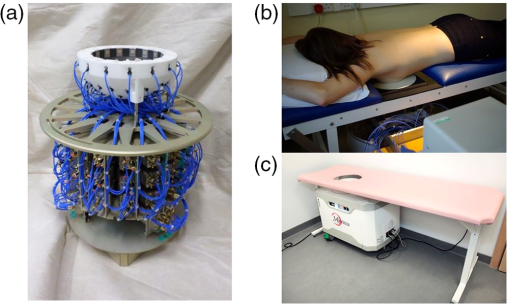
\includegraphics[width=0.5\textwidth]{MARIA_M4.png}
    \centering
    \caption{The MARIA M4 and M5 system. (a) The MARIA M4 antenna array. (b) The M4 in a clinical setting. (c) The integrated M5 package \cite{preeceMARIAM4Clinical2016}}
    \label{fig:MARIAM4}
\end{figure}

\noindent The team scanned 86 participants, with a mean age of 51.4 and a range of 24 - 78 years old. The M4 system showed a sensitivity of
74\% (64/86) when compared with the "gold-standard' of an ultrasound. The "sensitivity" was determined based on the
ability of the M4 system to localize a lesion as it correlated with the location in the ultrasound image. The research
team also divided the group into pre-/peri- and post- menopausal women and found that the sensitivity was 75\% and 73\%
respectively. However, the reliability of these results are called into question when considering the sample size of the
study. Given a sample size of 86, and assuming a normal distribution and that the results are statistically significant
($p < 0.05$, Z = 1.96), a 10.58\% margin of error was calculated. While this may not be enough to conclusively prove
that the M4 system is a viable alternative to Mammograms, it is enough to show promise. With a larger sample size, this
margin of error could be narrowed further.

\subsection{Wavelia}
The second system that was considered was the Wavelia Microwave Breast Imaging System developed by MVG Industries
\cite{moloneyWaveliaMicrowaveBreast2021}. The Wavelia system integrates the imaging system as well as the examination
bed into one complete package (Figure \ref{fig:WaveliaSystem}). The integrated package makes the Wavelia system an
appealing choice for some hospitals, however, its large size may be a barrier to adoption in some facilities where space
is a premium. \hfill \break

\begin{figure}
    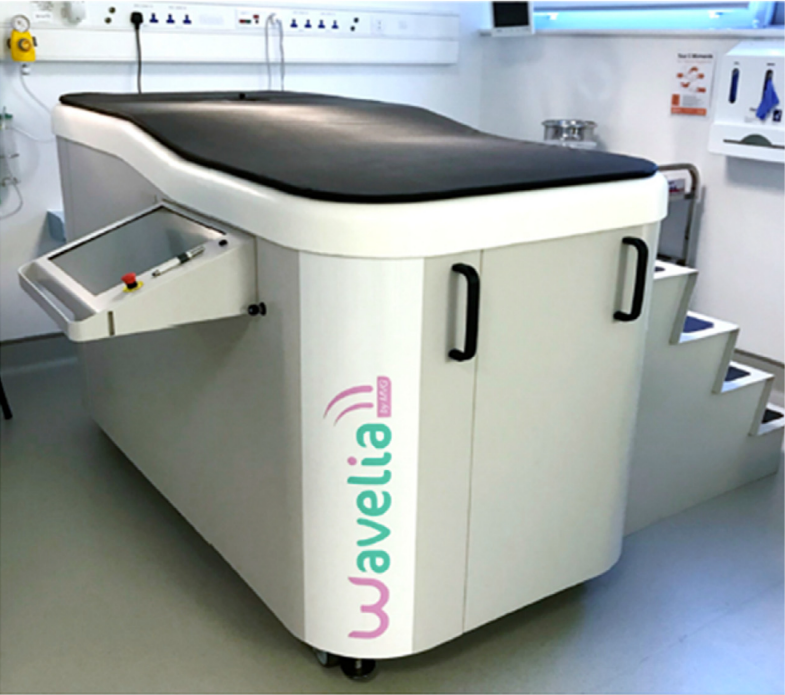
\includegraphics[width=0.5\textwidth]{Wavelia.png}
    \centering
    \caption{The Wavelia System \cite{moloneyWaveliaMicrowaveBreast2021}}
    \label{fig:WaveliaSystem}
\end{figure}

Like in the MARIA M4 system, patients lie in a prone position and place their breasts in the circular cutouts on the
bed. The system then begins to create a 3D reconstruction of the exterior of the breast using a stereoscopic camera.
This also allows for the breast volume to be explicitly calculated rather than being inferred like in the MARIA system.
The Wavelia makes use of the UWB spectrum when imaging the breast, although they opt for a narrower frequency range of
0.5 - 4.0 GHz compared to the 3.0 - 8.0 GHz range of the MARIA system. The antenna configuration, unlike the MARIA system, is an array of 18 Vivaldi-type probes arranged in a concyclic manner
on a horizontal plane. These antennas operate in a Multistatic manner and image the breast in sections parallel to the
coronal plane. The entire antenna assembly moves downwards in 5mm intervals to image the entire breast (Figure \ref{fig:LeveledMultistaticExample}). This is a
leveled multistatic system as opposed to the fully multistatic system in the MARIA M4. This leveled multistatic approach
has the benefit of a theoretically infinite vertical resolution. If the radiologist wanted a finer resolution along the
coronal plane, they would just have to tweak the array vertical step size, rather than having to manufacture an entirely
new antenna array, like in the MERIT system. This leveled approach also allows the parameters of the reconstruction
algorithm to be easily changed based on the particular section of the breast that we are imaging. The fully multistatic
approach, however, would need significant additional logic in the post-processing steps to determine which channels are
coplanar with a particular section. \hfill \break

\begin{figure}
    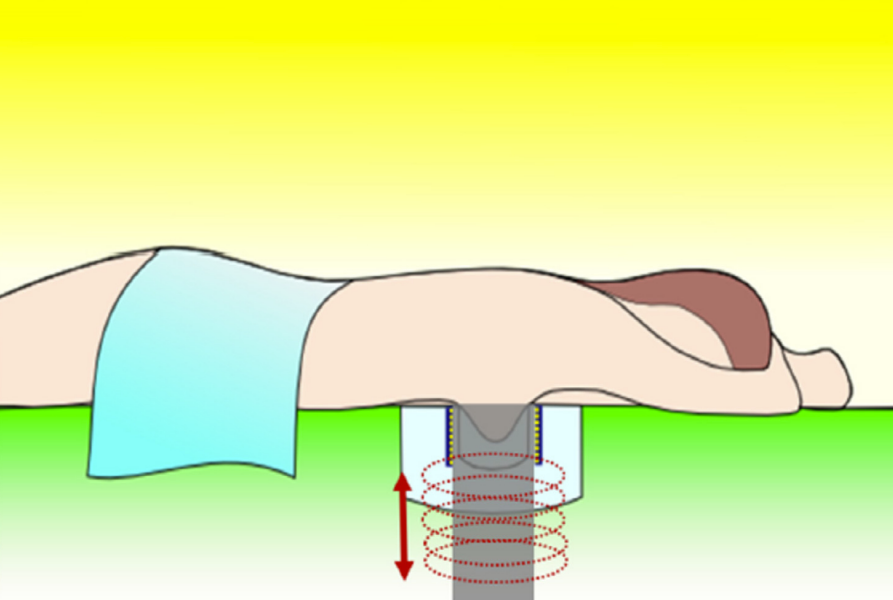
\includegraphics[width=0.5\textwidth]{LeveledMultistatic.png}
    \centering
    \caption{The Leveled Multistatic Approach of Wavelia \cite{moloneyWaveliaMicrowaveBreast2021}}
    \label{fig:LeveledMultistaticExample}
\end{figure}

\noindent The Wavelia paper \cite{moloneyWaveliaMicrowaveBreast2021} conducted a feasibility study on 25 female
participants. While the results aren't statistically significant, they do demonstrate the strengths of the Wavelia
system. 11 of the participants had a biopsy confirmed carcinoma and out of these, the Walia system detected 9 lesions,
with 7 being located to the appropriate region. Overall the system detected an abnormality in 21 of the 24 participants,
leading to a sensitivity of 87.5\%. The researchers do note some limitations of the Walia system, namely it can't detect
any lesions smaller than 10mm. This is significant since the size of the detected lesion plays a big factor when
deciding whether a lesion is cancerous or not. Another limitation of the system is that breast sizes that are too small
cannot be scanned in any great detail by the Wavelia system. Due to the patients being in the prone position, their
breast tissue needs to hang down far enough to have multiple sections of their breast be imaged by the antenna array.
The researchers are working on a subsequent system that should address all the aforementioned limitations. Overall the
participants had a positive outlook on the system. 23 out of the 25 women said that they would recommend the procedure
to other women and all of the women agreed that the information provided was clear and well understood.

\subsection{TSAR}
\setcounter{chapter}{2}
\setcounter{section}{0}
\chapter*{Julia}
\addcontentsline{toc}{chapter}{Julia}

\section{Why Julia?}
One of the goals of MERIT.jl was to streamline the development process for new imaging algorithms. As well as this
MERIT.jl aims to lower the barrier of entry and the coding knowledge needed in order to set up these data processing and
visualizing pipelines. In order to fulfill these dreams, the right coding language needed to be selected. Since the
barrier of entry needs to be low, a high-level language needs to be selected and since the primary target of MERIT.jl
are researchers, it needs to be a language that they are familiar with, or one which they can easily learn. If the
language chosen is too difficult to learn, any potential time savings from the ease of use would be heavily outweighed
by the time spent learning the language. \hfill \break

\subsection{Python}
Python was one of the languages considered. Python's philosophy was code readability over all and this fact is
complimented by its high-level syntax and indentation requirements. It was first introduced towards the end of the
1980's by Guido van Rossum and has had an expansive community ever since. The Python package repository and pip have
allowed the community to develop libraries that can be easily shared and downloaded. All these factors catapulted Python
into the limelight and it has become the go-to language for any data science and deep learning application. However,
several drawbacks severely limit the usability of Python for high performance applications. Firstly, Python is an
interpreted language, meaning that at runtime, the Python interpreter reads the Python file line by line and calls the
relevant machine code. Due to this interpretation step, raw Python code is slow to run. Due to this reason, most
performant libraries in Python tend to use C-optimized implementations behind the scenes. So in order to develop any
decently performing Python libraries, one also has to be proficient in C as well as know how to create C and Python
bindings. Secondly, the Python Interpreter makes use of a runtime lock known as the Global Interpreter Lock (GIL) which
makes parallel processing in Python incredibly difficult. The reason for the GIL comes down to Python's use of reference
counting for memory management. Reference counting is a method where each object in Python gets assigned a reference
variable that keeps track of the number of references that point to that object. As references to the object get
created, the count goes up, as references get deleted or reach the end of their scope, the count goes down. When the
reference variable reaches zero, this becomes a flag for the object to be deleted, since there are no longer any
references pointing to this object. In some threaded applications, this can cause some issues where the reference count
gets updated by multiple threads simultaneously. In some cases, this can cause the reference count to never reach zero
leading to a memory leak, or it can reach zero too early and the object gets removed. To get around this, Python puts a
lock on the interpreter itself, this is the GIL. This means that any Python bytecode needs to first acquire a lock on
the interpreter before it can be executed. This makes multithreading in Python incredibly difficult and slower than it
would be in other languages. So for these reasons, Python was rejected as the software of choice.

\subsection{MATLAB}
MATLAB was another language that was considered. Developed in 1984, it became the goto software for many research
purposes due to its ease of use and intuitive operations on matrices and its multi-dimensional analogues. It is taught
across every single engineering college, and one company estimates that MATLAB is being used in over 57,811 companies
\cite{CompaniesUsingMATLAB}. MATLAB, however, is still an interpreted language and therefore can be quite slow some
times. A study conducted by Aruoba and Fernández-Villaverde found that their MATLAB code ran about 3x slower than the
same code written in C++, highlighting just how big of a difference a compiler can make \cite{aruobaComparisonProgrammingLanguages2018}. It should be noted that the
MATLAB version of the code ran about 30.26x faster than the same Python code, implying that even though both are an
interpreted language, the MATLAB interpreter is much more optimized than the Python interpreter. But one of the biggest
drawbacks by far, is the fact that MATLAB is a license based language. In order to use MATLAB, one must pay a yearly
subscription of anywhere from €120 to €3,650 depending on the purpose for which it is used. This goes directly against
the open-source vision of MERIT.jl. This cost can become prohibitively expensive for small teams trying to work on new
systems and algorithms. Octave was briefly considered as it is a free and open-source competitor to MATLAB, but this
idea was quickly dropped when it became clear that Octave's main goal was compatibility with MATLAB scripts rather than
performance over MATLAB. For these reasons, MATLAB was also rejected as the software of choice.

\subsection{Julia}
The third and final language considered was the Julia programming language. Julia was developed by Jeff Bezanson, Stefan
Karpinski and Viral B. Shah, and was first released to the public in 2012. Julia was designed to be a coding language
that offered high-level syntax while also automatically compiling the code at runtime. Julia's Just In Time (JIT) compiler,
allows it to offer the full dynamism of Python and MATLAB while avoiding the drawbacks that come with having to use an
interpreter. The aforementioned study found that Julia was only 1.47x slower than the comparable C++ implementation.
Julia also offers features that are not in Python or MATLAB such as parametric polymorphism, multiple dispatch,
efficient garbage collection and a JIT that is capable of optimizations and ahead-of-time compilation. Julia also bakes
in native support for multiple parallel programming paradigms such as GPU programming and multithreading, making it an
appealing choice for people working on high-performance compute clusters. One other feature that made Julia wildly
popular was the native ability to call C and Fortran libraries without having to create any special wrappers. This "It
Just Works" ideology is what garnered Julia its well deserved popularity. With its rising fame and easy to understand
syntax, this was the coding language decided for MERIT.jl. In the next few sections, the various Julia features used
will be discussed in more detail. \hfill \break

\section{Features in Julia}
\subsection{Multiple Dispatch}
Multiple Dispatch is a programming paradigm in which a function can be dispatched (invoked) based not only on the
function name but also on the type and order of input arguments. This is opposed to the single dispatch
programming paradigm where the function that is dispatched usually depends on a special argument before the function
name. In almost all programming languages this is the variable name for that class. For example, consider the following
code: \hfill
\begin{lstlisting}
    Class Dog:
        name::string

        function says(a::string):
            print("The dog, $self.name says $a")
        end
    end

    Class Cat:
        name::string

        function says(a::string):
            print("The cat, $self.name says $a")
        end
    end

    billy = Dog("billy")
    kate = Cat("Kate")
\end{lstlisting}
If we wanted to call the "says" function for the Dog or Cat class, then we would have to write,
\lstinline|billy.says("Hello World")| or \lstinline|kate.says("Hello World")|. This is the single dispatch paradigm and
it is probably the one most people are familiar with. This fits well into an object-oriented programming language, where
objects are used to encapsulate concepts and ideas and therefore we create specialized functions that operate on the data
contained within that class. However, one drawback is that the compiler relies on the user to remember which
methods belong to which class, and also which methods are callable. Also, it isn't clear how one would write a function
that allows for the Cat and the Dog to interact with each other. Instead, now consider the multiple dispatch paradigm.
In Julia particularly, it is important to note that methods no longer belong to objects as we were forced to do in
single dispatch. Added to this, methods no longer have to be defined within the "class" but can be done after class
declaration or even class instantiation. Consider the example below: \hfill

\begin{lstlisting}
    struct Dog{
        name::string
    }

    struct Cat{
        name::string
    }

    function says(pet::Cat, a::string)
        print("The cat, $pet.name says $a")
    end

    function says(pet::Dog, a::string)
        print("The dog, $pet.name says $a")
    end    

    function encounter(petA, petB)
        print("$petA.name encounters $petB.name and $meets(petA, petB)")
    end

    function meets(petA::Cat, petB::Dog)
        return "hisses"
    end

    function meets(petA::Dog, petB::Cat)
        return "barks"
    end

    billy = Dog("Billy")
    kate = Cat("Kate")
    says(billy, "Hello")
    says(kate, "Hello")
    encounters(kate, billy)
    encounters(billy, kate)

\end{lstlisting}

Here we have a similar situation as before, but instead of having classes, we have structs and methods that take those
structs as arguments. On lines 30 and 31 in the code block above, we get a similar output as in single dispatch. But
where multiple dispatch really shines is in the next two lines. Here we have the cat and the dog encountering each
other. In single dispatch, someone would have to create a wrapper library to handle the interaction between two classes,
but in multiple dispatch it is as easy as creating another method. This can be seen in the "meets" functions defined in
the code block above. Since multiple dispatch relies on the input arguments as well, we can create specialized "meet"
functions for when a Dog meets a Cat or when a Cat meets a Dog. In the above code block executing line 32 would print
out "Kate encounters Billy and hisses". This is because we had a struct of type Cat as the first input argument to
"meets" and a struct of type Dog as the second argument. Line 33 on the other hand, would print "Billy meets Kate and
barks", since the order of the input arguments is reversed. Another notable consequence from this is that if anyone
else wanted to extend "meets" and therefore "encounters" to other animals, they would only need to define a struct with
the same fields as Cat and Dog, and new meets methods as such: \hfill

\begin{lstlisting}
    struct Rabbit{
        name::string
    }

    function meets(petA::Cat, petB:Rabbit)
        return "chases"
    end
    function meets(petB::Rabbit, petB:Cat)
        return "runs away"
    end

    kate = Cat("Kate")
    johnny = Rabbit(Johnny)
    encounters(kate, johnny)
    encounter(johnny, kate)
\end{lstlisting}

Line 12 in the above code block would print "Kate encounters Johnny and chases" while line would print "Johnny
encounters Kate and runs away". While these examples may be simple, they showcase the powerful flexibility and
extensibility behind multiple dispatch. It is this feature that allows all the Julia libraries to "just work" together,
without needing any glue-code. Some other developer could come along and create a new package for a "Lion" and so long
as it implements a struct with the same required field names as the other animals and creates a "meets" function, any
variable of type Lion will work well with the "encounters" function. 

\begin{figure}[!h]
    
\includegraphics[width=1\textwidth]{multipleDispatch.png}
    \centering
    \caption{Multiple Dispatch (top) vs Single Dispatch (bottom)} 
    \label{fig:multipleDispatch}
\end{figure}

\subsection{Type Heirarchy}
All the types in Julia are arranged in a tree-like structure and can be broadly classified into two categories, an
Abstract Type or a Concrete Type. Abstract types are the internal nodes of the type tree, having both parents and
children, while concrete types are the "leaves" of this tree. One notable difference between abstract types and concrete
types is that abstract types cannot be instantiated; they serve only as nodes in the type graph. While this may seem
pointless at first glance, it is this very feature that allows the multiple dispatch paradigm mentioned before to really
shine. Shown in Figure \ref{fig:juliaTypeHeirarchy}, is the type hierarchy for the Integer type, the abstract types are
highlighted in red, whereas the concrete types are highlighted in blue. \hfill
\begin{figure}[t]
    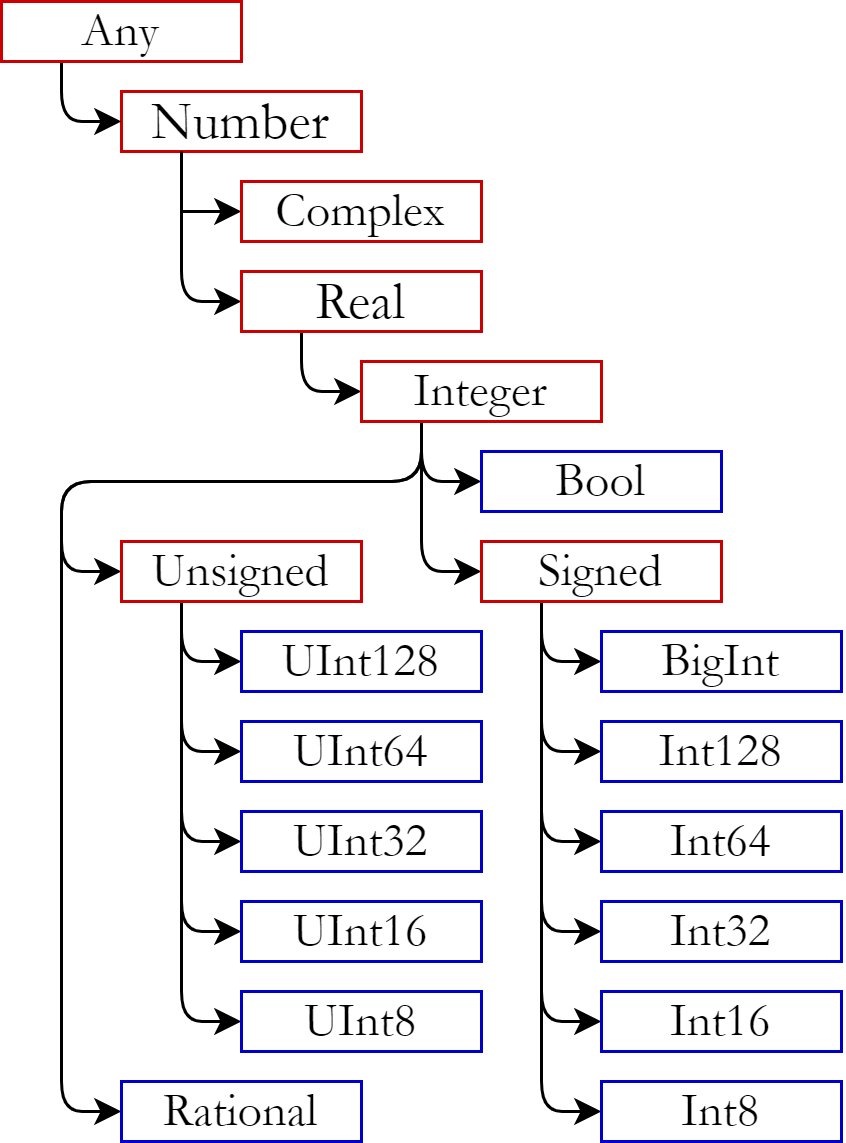
\includegraphics[width=0.45\textwidth]{juliaTypeTree.png}
    \centering
    \caption{Type hierarchy for the Integer Type} 
    \label{fig:juliaTypeHeirarchy}
\end{figure}

As well as giving us a way to logically organize types, the type hierarchy tightly integrates with the multiple dispatch
system. Consider for example the code block below: \hfill
\begin{lstlisting}[language=Julia]
    abstract type Animal end

    struct Cat <: Animal
        name::string
    end

    struct Dog <: Animal
        name::string
    end

    function encounters(petA::Animal, petB::Animal)
        verb = meets(petA, petB)
        println("$(petA.name) meets $(petB.name) and $(verb)")
    end

    meets(petA::Animal, petB::Animal) = "passes by."
    meets(petA::Cat, petB::Dog) = "hisses"
    meets(petA::Dog, petB::Cat) = "barks"

    whiskers = Cat("Whiskers")
    fudge = Dog("Fudge")
    encounters(whiskers, fudge)

    ####################################################
    #Defined in another library that subtypes the Animal abstract class.
    struct Rabbit <: Animal
        name::String
    end

    chomper = Rabbit("Chomper")
    encounters(whiskers, chomper)
\end{lstlisting}

In the above code block, we define an abstract Animal type, by default this is a subtype of the abstract type Any. Then
we define a concrete type Cat and a concrete type Dog. When line 22 gets executed, the multiple dispatch system will
choose the correct \lstinline[language=Julia]|meets()| function and "Whiskers meets Fudge and hisses", this is as expected. Now another developer
might want to implement a Rabbit type. So they create the Rabbit type as shown above, and specifies that it is a subtype
of the Animal abstract type via the \lstinline[language=Julia]{<:} operator. Even if they do not implement a
\lstinline[language=Julia]{meets()} that is specialized for their Rabbit class, the
\lstinline[language=Julia]{encoutners()} will still work since it only expects an input that is a subtype of Animal. The
\lstinline[language=Julia]{meets()} function will also work, since the original author implemented a
\lstinline[language=Julia]{meets()} method that accepts arguments of type Animal or any subtypes of it. But why didn't
the earlier call to \lstinline[language=Julia]{encoutners()} (and consequently \lstinline[language=Julia]{meets()})
fail, since both lines 15 and 16 are valid options for the dispatcher? This is an example of where multiple dispatch
benefits from having a type hierarchy. The Julia dispatcher always dispatches the function that is most specific across
\textbf{ALL} its arguments. So in the Cat and Dog case, the \lstinline[language=Julia]{meets()} on line 16 will be
dispatched. In the Cat and Rabbit case, the \lstinline[language=Julia]{meets()} one line 15 is the most specific
function and so that gets dispatched. This allows for amazing extensibility that isn't found in many other languages. Often
it is impractical for a developer to think of all the ways their library would be used or all the types or functions
that the end-users would require. In Julia, they don't have to think about it. Instead, they can define an abstract
class and some methods that accept the abstract class as inputs. The users can then create subtypes of this abstract
class and define their own methods for their new type. Neither developer has to be worried about whether they were through
enough to consider all possibilities, they can write code for their own purposes and trust that the Julia dispatcher and
type hierarchy would automatically determine the correct function to call. \hfill \break
This idea is heavily used in the MERIT.jl library. Currently, most of the research in microwave imaging is centered
around the breast and breast cancer, but in the future, this could be implemented for other body parts. As such, the
library needs to be flexible to allow for easy updates. MERIT.jl is centered around the Scan abstract type, from this
type we subtype the BreastScan type, which holds all the information from the scan of a particular breast. If in the
future microwave imaging gets used for a chest scan, all a developer would need to do is to implement a ChestScan
struct, subtyped from Scan, and implement a few functions and the Julia dispatcher will handle the rest. I, as the
original developer, do not need to worry about the intricacies of how a ChestScan struct would work, or what fields it
would need. I can trust that future developers can easily extend this library without introducing breaking changes to
the library core. In this way, MERIT.jl achieves extensive flexibility and expandability which would not be possible in
other languages.  \hfill \break

\begin{figure}[h]
    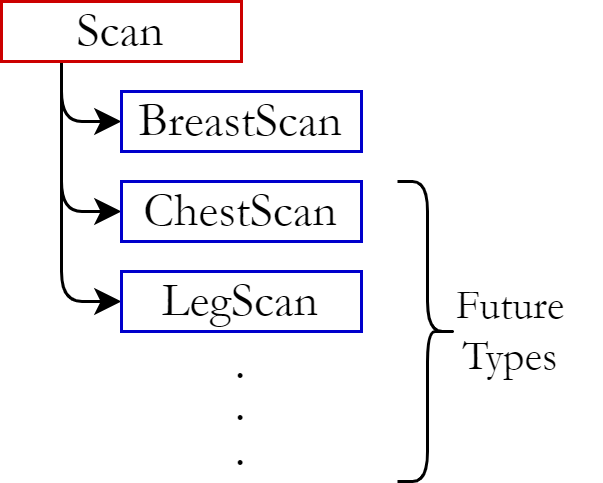
\includegraphics[width=0.45\textwidth]{scanType.png}
    \centering
    \caption{Current type hierarchy in MERIT.jl} 
    \label{fig:scanType}
\end{figure}

\subsection{Parametric Polymorphism}
Parametric polymorphism refers to the programming paradigm where a function can be created generic to the input argument
type. The compiler can then strongly type the function with the correct types. Consider the simple example of an
\lstinline[language=Julia]{addtwo(x)} function.

\begin{lstlisting}[language=Julia]
    function addTwo(x::T) where {T <: Real}
        return x + T(2)
    end
\end{lstlisting}

Instead of restricting x to a specific type, we replace it with the variable T and instead place a restriction on T. In
this case we say that T, and by extension x, can be any type that is a subtype of the abstract Real type. We also
convert the 2 from an Int64 type, to whatever type T is, to allow for accurate summation. If parametric polymorphism was
not a feature in Julia, this function would need to be duplicated 16 different times to account for all the concrete
subtypes of Real (see Figure \ref{fig:juliaTypeHeirarchy}). Parametric Polymorphism with the Julia type hierarchy allows
a developer to have incredible expressive power with very few lines of code. \hfill \break 
MERIT.jl uses this feature extensively due to the fact that the library needs to be agnostic to the type of the input
data. When instantiating the BreastScan struct the user can provide the types of the data that they will load and can
therefore set the internal data type of the struct. It would be impossible to support all 4,176 different permutations
of every single function, however, with parametric polymorphism, the function only needs to be defined once and the Julia
compiler will handle the rest. This means that researchers and developers don't have to worry about whether the library
functions can support the data type of their data, so long as it follows the type restriction set on the function, it
will produce an output, greatly simplifying the coding experience.  

\subsection{Type Stability}
Type Stability is a coding discipline that Julia recommends all code to use. A function whose contained variables have a
consistent type for the lifetime of that function is considered to be "type stable" or to have "type stability". Another
way to think about this is that if the output type only depends on the input types, then the function is type stable.
Consider the following two functions: \hfill
\begin{lstlisting}[language=Julia]
    function unstable()
        x = 1
        for i = 1:10
            x /= rand()
        end
        return x
    end
    
    function stable()
        x = 1.0
        for i = 1:10
            x /= rand()
        end
        return x
    end
    
\end{lstlisting}
In both functions, we have a variable x which gets divided by a random float 10 times, with the result being returned.
However, the first function is considered to be type unstable while the second function is type stable. This is because
in the first function x was declared as an Int64, but when we divide by the random Float64, the data type of x changes
to Float64 as Julia performs floating point division by default. Whereas in the second function, x gets declared as a
Float64 and remains as a Float64 when it gets returned. Type Stability is important because if the Julia compiler can
determine that the types of the variables stay constant for the lifetime of the function, it can perform optimizations
on the machine code that would otherwise be impossible. These optimizations are evident when benchmarking the functions
above. Using the \lstinline[language=Julia]{@benchmark} macro from BenchmarkTools, I timed both functions. They were run
multiple times to ensure that only the compiled versions of the function were being executed rather than the functions
being interpreted. The benchmarks showed that on average the type stable function ran in 306.178ns whereas the type
unstable function ran in 573.355ns; almost 1.87x slower. When considering the many hundreds of function calls required
to produce an output in MERIT.jl, these slowdowns become significant. When coding functions for MERIT.jl, I aimed to
preserve type stability in functions that I knew would be called frequently. The
\lstinline[language=Julia]{@code_warntype} macro was greatly beneficial in this task as it flags sections of code where
the compiler cannot definitively infer the type of a variable or where it suspects there might be some type instability.
Having type stable functions in MERIT.jl was a necessity, where possible, due to the large datasets that need to be processed. An 8cm
radius breast at 0.25cm resolution has about 70k points, which need to have their distances to each antenna calculated.
Assuming we are dealing with the MARIA M4 system with its 60 antennas, this equates to around 4.2M distance calculations
alone for each image. Running such calculations on type unstable functions would be prohibitively expensive and would
take far too long to compute. Herein lies one of the drawbacks of using the Julia language. While the dynamism offers us
powerful expressibility, it also comes at the cost of massive slowdowns when used incorrectly. While it may be easy to
create type stable functions for the example shown in the code block above, it becomes increasingly harder to create
type stable code when the operations that need to be performed become more complex. Creating performant code in these
situations requires the developer to have advanced knowledge of the language. This does raise the barrier of entry for
people who want to contribute to the library. However, I feel that this is an acceptable trade-off since the benefits
that come from having a performant library, such as increased usage and better recognition, far outweigh the negatives
from having an increased barrier of entry.

\subsection{Closure}
Closure in programming refers to the practice of calling a function A which returns a function B that has some
information about the variables in the scope of function A. Consider the following simple example:
\begin{lstlisting}[language=Julia]
    function addX(x)
        scalar = x

        function calc_(a)
            return a + scalar
        end
    end

    add5 = addX(5)
    add7 = addX(7)
    add5(2)  # Will return 7
    add7(10) # Will return 17
\end{lstlisting}
Here a function called \lstinline[language=Julia]{addX} is defined which accepts an input \lstinline[language=Julia]{x},
assigns it to a variable called \lstinline[language=Julia]{scalar} and finally defines a function called
\lstinline[language=Julia]{calc_} which calculates and returns \lstinline[language=Julia]{a + scalar}. Here we say that
\lstinline[language=Julia]{scalar} is "captured" by \lstinline[language=Julia]{calc_}. When calling the
\lstinline[language=Julia]{addX} function as was done in line 8, we receive a function pointer of sorts to a
parametrized \lstinline[language=Julia]{calc_}. Note that by default Julia automatically returns the last thing computed
in the executed function's scope, this is how \lstinline[language=Julia]{calc_} is returned from
\lstinline[language=Julia]{addX} without an explicit return statement. This idea of closure is important as it allows
users to customize parametric functions to suit their particular needs. The MERIT.jl library uses this in the
\lstinline[language=Julia]{get_delays} function in the Beamform.jl file (for more information see the GitHub link in
the Introduction). Earlier sections showed
how $epsilon$ is a free parameter in the beamforming equations, one that researchers would be changing frequently.
Implementing closure for the \lstinline[language=Julia]{get_delays} method allows researchers to quickly and easily
define a set of delay functions which they can pass to the \lstinline[language=Julia]{beamform} function to see the
various effects on the resulting scan that come from tweaking $epsilon$. This fulfills one of the other tenets of the
library, which was to create an interface that allowed for flexibility and customizability in the functions that
mattered. One important thing to keep in mind is that captured variables must never be reassigned otherwise, the
compiler will not be able to infer the data type of the variables leading to slow and type unstable code. Again this
highlights one of the draw backs of using Julia, writing customizable code is relatively easy, however writing code that
is both customizable and performant is tough. Any researcher who might want to implement a custom delay function (e.g.
one that does not assume a straight line model) using closure, would have to make frequent use of the
\lstinline[language=Julia]{@code_warntype} to ensure that the code they have written is type stable, and therefore comes
with some promises of performance.  

\subsection{Type Safety}
Type Safety refers to a program or language's ability to detect and discourage errors that arise from performing
operations on the wrong data type. For example in Julia, one can easily add two numeric types together but if one tried
to add two strings together, the Julia compiler would produce an error, since that would be an illegal operation. This
offers some level of protection against illegal operations, but there are many cases where the type of the variable
agrees with the operation being performed, but their semantic meaning disagrees. Consider the example of a function used
to calculate the speeds of various vehicles. The function \lstinline[language=Julia]{calcSpeed} accepts a vector for
distance traveled by the various cars and the times each car took to travel that distance and returns the speed of each
car in a third vector.

\begin{lstlisting}[language=Julia]
function calcSpeed(dist::Vector{T}, t::Vector{T}) where {T <: Real}
    return dist ./ t
end

#################################################### 
distance = rand(1, 100)
time = rand(1, 100)
calcSpeed(distance, time)   # Will compute the speed

#################################################### 
distance = rand(1, 100)
time = rand(ComplexF64,1, 100)

# Will throw an error since there is a type mismatch
calcSpeed(distance, time)  

#################################################### 
distance = rand(1, 100)
time = rand(1, 100)

# Will compute the wrong answer, but no error gets thrown
calcSpeed(time, distance) 
\end{lstlisting}
On line 8, calcSpeed gets called correctly and returns the speed of each car correctly. On line 13, the Julia compiler
will throw an error because the \lstinline[language=Julia]{time} variable is a Complex Float64 and
\lstinline[language=Julia]{calcSpeed} only accepts types that are a subset of Real. However, on line 18, no error is
thrown even though the wrong answer is returned. This is because compilers can only make deductions on the concrete
types of the variables and the operations being performed and not on the semantic meaning of the function, variable
names and what it means to call the function with those variables. However, we can limit the chance of a variable being
passed to the wrong positional argument by creating lightweight types that encode this semantic information in their
type name. In the above case, it would mean creating a "distance" type, and a "time" type that are wrappers around some
in-built concrete type. With this, the compiler will throw an error when running line 18 as the function received a
vector of type "time" when it was expecting one of type "distance". \hfill \break
The MERIT.jl library exemplifies the idea of "strong" type safety through its implementation of the Point
data type. The Point type is an abstract type from which the Point3 and Point2 concrete type subsets. These are
lightweight wrappers around a grouping of 3 and 2 numbers respectively and serve the purpose of being a 3D and 2D point.
\begin{lstlisting}[language=Julia]
    abstract type Point end

    # xyz can be any data type that is a subset of Real
    mutable struct Point3{T <: Real} <: Point
        x::T
        y::T
        z::T 
    end

    mutable struct Point2{T <:  Real} <: Point
        x::T
        y::T
    end
\end{lstlisting}
Since these are custom data types, the inbuilt operators could not be used on them. So in addition to this, MERIT.jl
also had to extend some of the inbuilt operators using the concepts from parametric polymorphism so that these points
data types could be used in a meaningful way. For the full suite of operations implemented, please refer to the GitHub
link in the Introduction. Every other function in the library that needs to work with the points from the imaging domain,
e.g. the \lstinline[language=Julia]{domain_hemisphere!} and the \lstinline[language=Julia]{get_delays}, to name a few,
accept collections of the points data types rather than simply accepting a matrix of numbers. This way, an error gets
thrown if any other collection of numbers that is not a points data type is passed in that argument. This does not
entirely solve the problem however, it is still feasible for a Point3 variable representing antenna locations to be
mistakenly used in the place of a Point3 variable which describes the imaging domain. Even though this issue still
exists in some part, the hope is that with this new type, the chance of the aforementioned issues arising would be
minimal. 

%% Talk about performance impact about new points type execution time went from 8 to 12 seconds.

Due to time constraints, the entire library could not be made strongly type safe, but the Points.jl file
provides an excellent template that could be used to implement further types to eventually reach a strong type safety
that is in every function in the library.

\subsection{Customizability}
The customizability of the MERIT.jl library has been demonstrated extensively in the previous sections. However, nowhere
is this exemplified more than in the BreastScan struct. The entire library is built around the use of the Scan structs.
These structs encapsulate all the information about a particular Scan, including all the required information about the
machine that was used to conduct the scan. Most importantly each scan struct is recommended to have two function pointer
fields which will hold pointers to the delay function and the beamforming function to be used in the beamforming
process. During the setup process, researchers can easily swap out the delay function or the beamforming function used
by overwriting these function pointers with other relevant functions from the library or with their own functions. In
order to work with the one-call data processing pipeline in MERIT.jl, researchers just need to ensure that their delay
and beamformer functions follow these templates:
\begin{lstlisting}[language=Julia]
    function delay_template(relative_permiativity)
        #Capture the relatively_permiativity
            function(channels, antenna, domain_points):
                #calculate and return a time matrix
                #Size = (1 x #Channels x #Points)
            end
    end
    
    function beamformer(delayed_signals)
        #Do some processing
        #return should be of size (1 x 1 x #Points)
    end
\end{lstlisting}
These templates allow for a lot of flexibility and are really where MERIT.jl shines in comparison to its MATLAB counter
part. Researchers who just want to benchmark new algorithms against already established ones just need to follow these
templates and they can be guaranteed that their functions will "just work" with the one-call data processing pipeline.
If their functions also follow the rules of type stability mentioned above, they can also have some reasonable
guarantees that any slowdowns are caused by their implementations rather than the lack of compiler optimizations for
type unstable code. 
\setcounter{chapter}{2}
\setcounter{section}{0}
\setcounter{subsection}{0}
\chapter*{Programming Paradigms}
\addcontentsline{toc}{chapter}{Programming Paradigms}
As mentioned in the section before, Julia's development was centered around the philosophy of creating a dynamic yet high
performing language by combining features like Multiple Dispatch and Parametric Polymorphism among others. The following
sections will describe a small subset of these features.

\section{Multiple Dispatch}
Multiple Dispatch is a programming paradigm in which a function can be invoked based not only on the function name but
also on the type and order of input arguments. This is opposed to the single dispatch programming paradigm where the
function dispatched depends on a special argument placed before the function name. In almost all programming languages
this is the variable name for that class. For example, consider the following code: \hfill
\begin{lstlisting}[language=Julia]
# Defined in one library
Class Dog:
    name::string
    function says(a::string):
        print("The dog, $self.name says $a")
    end
end

billy = Dog("Billy")

# Defined in another library
Class Cat:
    name::string
    function says(a::string):
        print("The cat, $self.name says $a")
    end
end

kate = Cat("Kate")
\end{lstlisting}
If one wanted to call the \lstinline[language=Julia]{says} from the Cat or Dog class in the single dispatch paradigm,
one would have to write \lstinline[language=Julia]{billy.says("Hello World")} or
\lstinline[language=Julia]{kate.says("Hello World")}. This concept fits well with object-oriented programming languages
where classes are used to encapsulate concepts. However, a drawback of this system is that the compiler relies on the
user to remember which methods belong to the class and which methods are callable. Also since both the Cat and Dog
classes are defined in different libraries it is not clear how either developer could create a function where these
classes interact with each other without having to create a separate third library that implements compatibility code.

Multiple and its particular implementation in Julia solves some of these issues. In Julia, methods no longer belong to
classes, instead like in C they simply belong to a particular library, also known as a ``Module'' in Julia. Functions
defined in modules are usually exported such that they are available in the namespace of any other module that uses it.
This allows modules to use and overload functions and structures from other modules in a way that is completely
transparent to the end user.   
\begin{lstlisting}[language=Julia]
# Defined in library A
struct Dog{
    name::string
}

function says(pet::Dog, a::string)
    print("The dog, $pet.name says $a")
end  

# Defined in library B 
struct Cat{
    name::string
}

function encounters(petA, petB)
    print("$petA.name encounters $petB.name and $meets(petA, petB)")
end

function meets(petA::Cat, petB::Dog)
    return "hisses"
end

function meets(petA::Dog, petB::Cat)
    return "barks"
end

# Overloading function from library A
function says(pet::Cat, a::string)
    print("The cat, $pet.name says $a")
end


# Someone else using both libraries
billy = Dog("Billy")
kate = Cat("Kate")

says(billy, "Hello World")
says(kate, "Hello World")

encounters(kate, billy)
encounters(billy, kate)
\end{lstlisting}
In the above code block, library B overloads the \lstinline[language=Julia]{says} function to accept a struct of type
Cat. In addition to this, it also creates two new \lstinline[language=Julia]{meets} functions that handle the
interaction between the Cat and the Dog types, as well as an \lstinline[language=Julia]{encounters} function. A third
user can make use of both libraries as they did in the single dispatch case, but now they only have to call the function
name, rather than the function name prepended with the class variable name. In the case of the
\lstinline[language=Julia]{says} function call, the Julia compiler automatically dispatches the correct implementation
based on the type of the input argument. This is further exemplified in the final two function calls. As stated before
multiple dispatch is sensitive to both the type and order of the inputs. In the first call to the
\lstinline[language=Julia]{encounters} function, the \lstinline[language=Julia]{meets} function on line 19 will be
dispatched as the argument order was of type Cat and then Dog. Whereas in the second call to the
\lstinline[language=Julia]{encoutners} function, the \lstinline[language=Julia]{meets} function defined on line 23 will
be dispatched due to the reverse ordering of the types.

\begin{figure}[!h]
    
\includegraphics[width=1\textwidth]{multipleDispatch.png}
    \centering
    \caption{Multiple Dispatch (top) vs Single Dispatch (bottom) demonstrating that in the multiple dispatch paradigm, the executed function also depends on the type and order of its inputs} 
    \label{fig:multipleDispatch}
\end{figure}

\section{Type Heirarchy}
In Julia, all types are arranged in a tree-like structure and can be broadly classified into two categories, an Abstract
Type or a Concrete Type. Abstract types are the internal nodes of the type tree, having both parents and children, while
concrete types are the ``leaves'' of the tree, having parents but no children. Another notable difference between
abstract types and concrete types is that abstract types cannot be instantiated, they serve only as nodes in the type
graph. Shown in Figure \ref{fig:juliaTypeHeirarchy}, is the type hierarchy for the Integer type, abstract types are
highlighted in red, whereas concrete types are highlighted in blue. \hfill
\begin{figure}[t]
    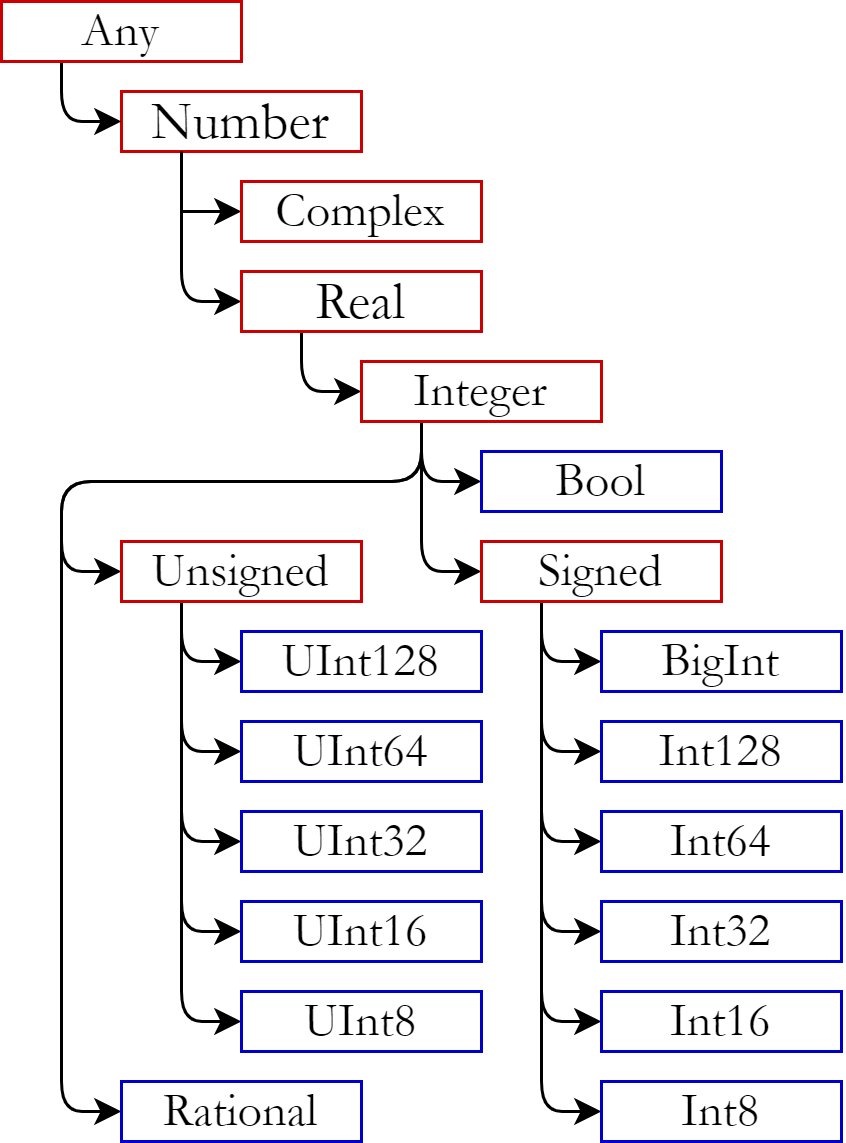
\includegraphics[width=0.45\textwidth]{juliaTypeTree.png}
    \centering
    \caption{Type hierarchy for the Integer Type} 
    \label{fig:juliaTypeHeirarchy}
\end{figure}
\FloatBarrier
The type hierarchy not only provides a way to logically organize types but also tightly integrates with the multiple
dispatch system mentioned before. It is this pairing that allows Julia to fulfill its promise of easy and powerful
extensibility. The following example helps illustrate this further.
\begin{lstlisting}[language=Julia]
# Defined in library A
abstract type Animal end

struct Cat <: Animal
    name::string
end

struct Dog <: Animal
    name::string
end

function encounters(petA::Animal, petB::Animal)
    verb = meets(petA, petB)
    println("$(petA.name) meets $(petB.name) and $(verb)")
end

meets(petA::Animal, petB::Animal) = "passes by."
meets(petA::Cat, petB::Dog) = "hisses"
meets(petA::Dog, petB::Cat) = "barks"

# Defined in library B
struct Rabbit <: Animal
    name::String
end

whiskers = Cat("Whiskers")
chomper = Rabbit("Chomper")
encounters(whiskers, chomper)
\end{lstlisting}
Library A defines a type hierarchy with Cat and Dog being a subtype of the abstract Animal type. The library then
implements a series of \lstinline[language=Julia]{meets} functions and an \lstinline[language=Julia]{ecounters}
function, similar to the example in the previous section. However, unlike the example before, there is a new
\lstinline[language=Julia]{meets} which accepts an argument of type Animal. Library B, importing library A, defines a
Rabbit type that is a subtype of the Animal abstract type and then calls the encounters function from library A. The
dispatch system cannot execute the \lstinline[language=Julia]{meets} function from lines 18, since
\lstinline[language=Julia]{chompers} is not of type Dog. Instead, it executes the \lstinline[language=Julia]{meets}
function on line 17, since both \lstinline[language=Julia]{whiskers} and \lstinline[language=Julia]{chompers} are valid
Animal types. This highlights an important interplay between the type hierarchy and the multiple dispatch system, in
that when dispatching, the Julia compiler will select the function that is most specific across all its input arguments.
The developer of library A need not worry about all the other possible Animal types, or what their fields may contain,
they can create a generic \lstinline[language=Julia]{meets} function that accepts any subtype of the Animal class and
will execute successfully provided the subtyped class contains the fields being accessed. Neither developer has to worry
about the completeness of the other's implementation, provided developer B follows the standards set by developer A,
they can develop an extension to library A and trust that the two libraries will be comparable.

\section{Parametric Polymorphism}
Parametric polymorphism refers to the programming paradigm where a function can be made generic to the input argument
type. At compilation time, the compiler can strongly type the function based on the types of the input arguments.
Consider the simple example of an \lstinline[language=Julia]{addtwo(x)} function.
\begin{lstlisting}[language=Julia]
function addTwo(x::T) where {T <: Real}
    return x + T(2)
end
\end{lstlisting}
Instead of specifying a concrete type for \lstinline[language=Julia]{x}, it is parametrized by the variable
\lstinline[language=Julia]{T} which has an abstract type restriction on it. This implies that
\lstinline[language=Julia]{T}, and by extension \lstinline[language=Julia]{x}, can by any type that is a subtype of the
Real abstract type. If parametric polymorphism was not a Julia feature, this function would have to be duplicated 16
times to account for the various concrete types that are a subtype of Real (see Figure \ref{fig:juliaTypeHeirarchy}).

\section{Type Stability}
\label{TypeStability}
Type Stability is a coding discipline that Julia recommends all code use. A function whose contained variables have a
consistent type for its lifetime is considered to be ``type stable'' or to have ``type stability''. Another way to think
about this, is that if the output type depends only on the input types, then the function is type stable. Consider the
following two functions: 
\begin{lstlisting}[language=Julia]
function unstable()
    x = 1
    for i = 1:10
        x /= rand()
    end
    return x
end

function stable()
    x = 1.0
    for i = 1:10
        x /= rand()
    end
    return x
end
\end{lstlisting}
Both functions have a variable, \lstinline[language=Julia]{x} which is divided 10 times by random floats and is returned
at the end of the function. However, based on the description above, the first function is considered to be ``Type
Unstable'' whereas the second function is considered to be ``Type Stable''. This is because in the first function the
type of \lstinline[language=Julia]{x} changes in the lifetime of the function (turns from Int64 to Float64). However in
the second function, the data type of \lstinline[language=Julia]{x} stays as a Float64 throughout the lifetime of the
function. The notion of type stability is important as it allows the Julia compiler to perform optimizations based on
the known data type of the variables at compile time. For type unstable functions, their unstable variables default to
type Any, ergo forgoing any optimizations. These optimizations are evident when benchmarking the functions above. This
was performed using the \lstinline[language=Julia]{@benchmark} macro from the BenchmarkTools module. Both functions were
run multiple times to ensure that only the compiled versions of the functions were executed rather than the interpreted
version. These benchmarks showed that on average the type unstable function ran 1.87x slower than the type stable
function (573.355ns and 306.178ns respectively).  

\section{Closure}
Closure in programming refers to the practice of calling a function A that returns a function B which has some
information about the variables contained in the scope of function A. Consider the following simple example:
\begin{lstlisting}[language=Julia]
function addX(x)
    scalar = x
    function calc_(a)
        return a + scalar
    end
end

add5 = addX(5)
add7 = addX(7)

add5(2)  # Will return 7
add7(10) # Will return 17
\end{lstlisting}
Defined above is a function called \lstinline[language=Julia]{addX} which accepts an input \lstinline[language=Julia]{x}
and assigns it to a variable \lstinline[language=Julia]{scalar}, before constructing and returning the function
\lstinline[language=Julia]{calc_}. This can be beneficial as it allows developers to create a family of functions that
are parametrized by their input variable.  It must be noted that the
captured variable, in the above case \lstinline[language=Julia]{scalar}, must never be reassigned, otherwise, the
compiler will not be able to infer the data types leading to type unstable code, and by extension all the negative
consequences mentioned in the previous section.

\section{Type Safety}
Type Safety refers to a program or language's ability to detect and discourage errors that arise from performing
operations on the wrong data type. For example in Julia, it is simple to add two numeric types, but performing the same
operation on two strings would yield an error, since the summation operator is not defined for two string types. This
offers some level of protection against illegal operations, but there are many cases where the type of the variables
agree with the operation being performed, but their semantic meaning disagrees. The example below will illustrate this
idea.
\begin{lstlisting}[language=Julia]
function calcSpeed(dist::Vector{T}, t::Vector{T}) where {T <: Real}
    return dist ./ t
end

#################################################### 
distance = rand(1, 100)
time = rand(1, 100)
calcSpeed(distance, time)   # Will compute the speed

#################################################### 
distance = rand(1, 100)
time = rand(ComplexF64,1, 100)

# Will throw an error since there is a type mismatch
calcSpeed(distance, time)  

#################################################### 
distance = rand(1, 100)
time = rand(1, 100)

# Will compute the wrong answer, but no error gets thrown
calcSpeed(time, distance) 
\end{lstlisting}
In the code block above \lstinline[language=Julia]{calcSpeed} accepts a vector of distance and time and returns the
associated speeds. Executing line 8, as expected returns the calculated speeds correctly. Executing line 12 will throw a
type error since ComplexF64 is not a subtype of Real. Line 22 however, will execute and return successfully even though
the wrong answer is returned, as the arguments were provided in the wrong positional order. This is because compilers
can only make inferences regarding the legality of a statement based solely on the concrete types of its arguments
rather than their semantic meaning in the context of the function being executed. However, the chance of variables being
incorrectly passed positionally can be negated by creating lightweight types that encode this semantic information in
their type name. In the above case, it would mean creating a ``distance'' type and a ``time'' type that act as wrappers
around a numerical concrete type. This way when line 22 is executed, instead of returning an incorrect answer, the
compiler will raise an error as the ``time'' and ``distance'' types were provided in the wrong order.
\setcounter{chapter}{4}
\setcounter{section}{0}
\setcounter{subsection}{0}
\chapter*{Results}
\addcontentsline{toc}{chapter}{Results}
\section{Current Workflow}
\label{CurrentWorkflow}
The current workflow in MERIT.jl was designed to be simple and approachable without much background knowledge about how
Julia or the underlying library works. Shown below is the full workflow needed to generate a plot from the data:
\lstinputlisting[language=Julia]{../../src/GettingStarted.jl}
A user would first instantiate the BrestScan struct and assign the data types that would be used throughout the
processing pipeline. The first type sets the data type and thereby the precision of the points composing the imaging
domain, the antenna locations and the frequency divisions. This can be any datatype that is a subset of type Real. The
second type controls the data type of the signal matrix containing the data collected from each antenna. This can be any
type that is a subtype of Number allowing for time-domain (Real) signals or frequency-domain (Complex) signals. The
third type controls the data type of the channels, and it can be any type that is a subtype of Integer. The choice of
data type here has no accuracy impact on the final result and it is recommended to choose an Unsigned Integer data type
that is big enough to index all the antennas. The next step would be to generate the imaging domain, this is
accomplished using the \lstinline[language=Julia]{domain_hemisphere!} function. This accepts the resolution and the
assumed or calculated radius of the breast. The user would then have to make use of the
\lstinline[language=Julia]{load_XXX!} functions to load the data into the relevant fields of the struct. These functions
assume the data is contained in a CSV file and contain no headers. The user then populates the relevant fields with
their chosen beamformer and delay function. At this stage, the user can then pass the whole struct to the
\lstinline[language=Julia]{beamform} which will beamformer the provided signals into a set of data that can then be
visualized as demonstrated towards the end of the code block above. Overall the entire workflow can be seen in Figure
\ref{fig:MERITWorkflow}.

\begin{figure}[h!]
    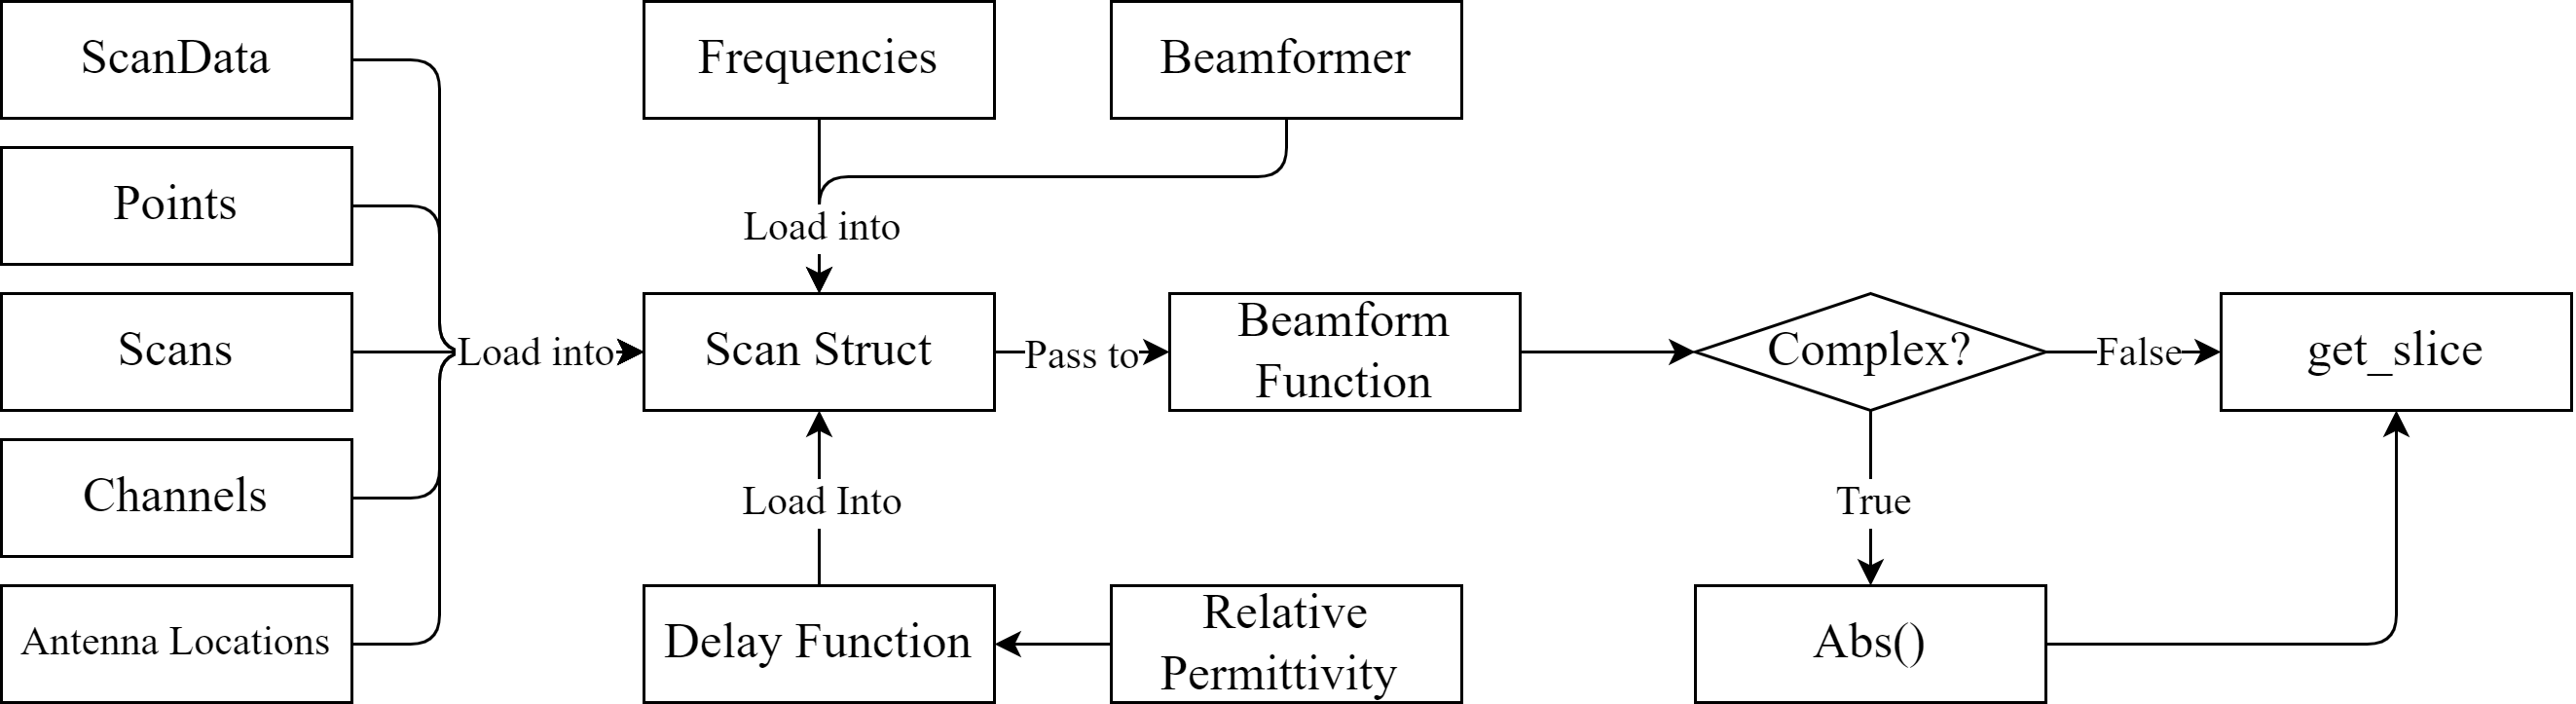
\includegraphics[width=1\textwidth]{MERITWorkflow.png}
    \centering
    \caption{An overview of the current workflow used to image a scan in MERIT.jl} 
    \label{fig:MERITWorkflow}
\end{figure}

This workflow exemplifies how easy it is to use the MERIT.jl library. The function names were deliberately chosen to be
verbose and conform to established nomenclature in the field so that anyone who wants to use the library can understand
what each function does without having to delve into the source code. In this way, the MERIT.jl library is somewhat self
documenting. Additional information is provided above each function in the form of docstrings which can be used with the
help function built into the Julia REPL. This was done in a bid to lower the prerequisite knowledge needed to use the
library, thereby fulfilling one of the goals of MERIT.jl which was to create an open and accessible library. 

\section{MERIT.jl Results}
The library was benchmarked against the MATLAB implementation created by Dr. O'Loughlin \textit{et al.} to ensure that the
results provided by MERIT.jl are provably correct. Both implementations were given the same data, B0\_P3\_p000.csv and
B0\_P3\_p036.csv. Rotational subtraction was performed on these in both libraries to reduce the presence of skin
reflections in the data as mentioned before. The data was then processed according to the processing pipeline
recommended by both libraries, the result of which can be seen below in Figure \ref{fig:OutputResults}. It should be
noted that the \lstinline[language=Octave]{imshow} function was used in MATLAB to plot the image. This had the effect of
reflecting the image across the x-axis and also slightly stretching the image along the x-axis, however, the matrix
holding the image data still shares the same layout as the image matrix in Julia so a numerical comparison between the
two could be performed. The averaged MSE proved to be an excellent choice as a numerical comparator, due to the squaring
operations in the MSE formula any small differences would be greatly magnified in the error. This is desirable when the
goal is to see if MERIT.jl can provide output that is similar to its MATLAB counterpart. Computing the averaged MSE
between the two images yielded an error of $8.4417 \times 10^{-7}$ which is well within the accuracy of a float, making
it effectively identical to the images produced by MATLAB. This shows that the Julia library in its current state
provides a viable alternative to the MATLAB implementation for frequency domain analysis.

\begin{figure}[t]
    \begin{tabular}{cc}
        \subfloat[MERIT.jl Output]{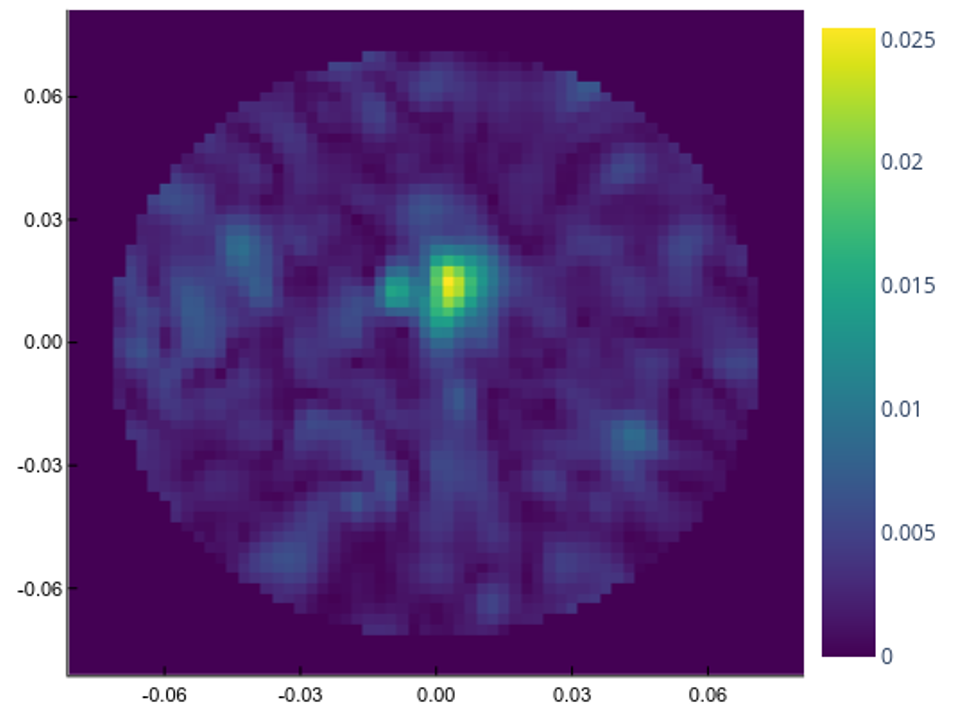
\includegraphics[width=0.45\linewidth]{JuliaOutput.png}}&
        \subfloat[MATLAB Output]{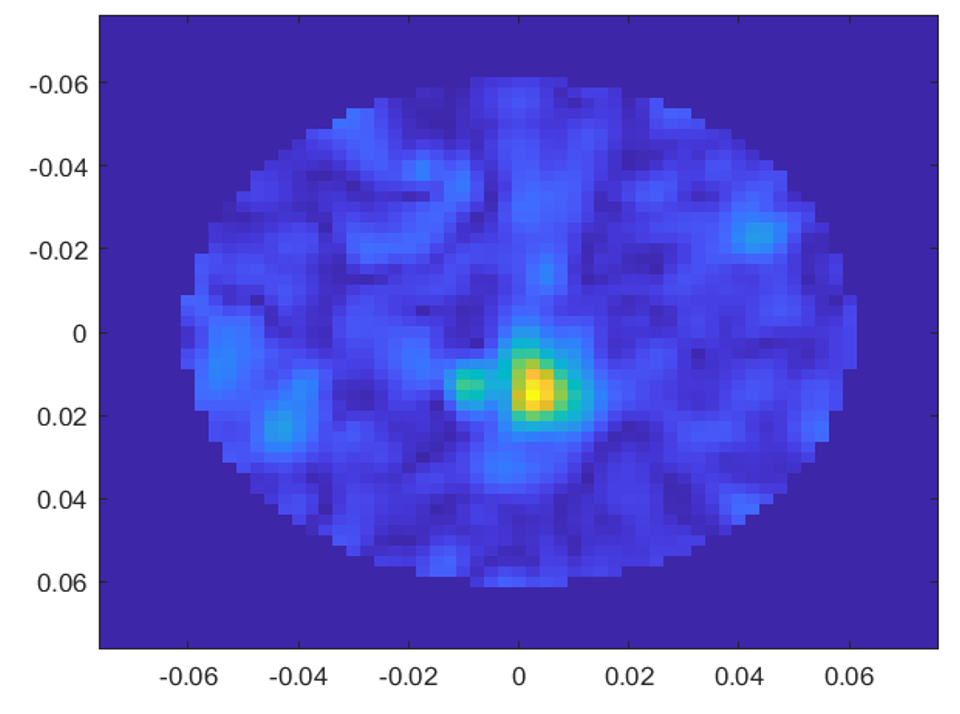
\includegraphics[width=0.45\linewidth]{MATLABOutput.png}}
    \end{tabular}
    \caption{A comparison between Julia and MATLAB output, showing an averaged MSE of $8.4417 \times 10^{-7}$}
    \label{fig:OutputResults}
\end{figure}

\section{Performance of MERIT.jl}
One of the requirements for MERIT.jl was that it had to be performant. Through the use of type stability, SIMD optimized
for loops and the disabling of array bounds checking, the library could process the provided data in 8 seconds. However,
after the addition of the Points data type for type safety, the processing time climbed to 12 seconds. While the overall
runtime is still acceptable, an increase of 3 seconds is less than ideal. While no official analysis has been conducted
to narrow down the cause of the slowdowns, I suspect that perhaps it may be down to unoptimized implementations of the
basic operators such as addition and squaring in the Points.jl library. It should also be noted that when running the
library, my laptop constantly ran into memory limits and had to write some memory to a swap file on disk. I believe that
moving memory in and out of this file might also be partly responsible for the increased runtime, however, further
research is necessary to determine a definitive cause. To capture the full performance characteristics of the library, a
scalability test was performed, in which the number of points, channels and frequency divisions were progressively
increased. This was performed in an automated manner using the functions provided by BenchmarkTools.jl
\cite{BenchmarkToolsJl}. The results from the benchmark suites were then exported to CSV files and analyzed in Excel to
judge the ``Big O'' notation of MERIT.jl.

\begin{figure}[h!]
    \begin{tabular}{cc}
        \subfloat[Raw Points]{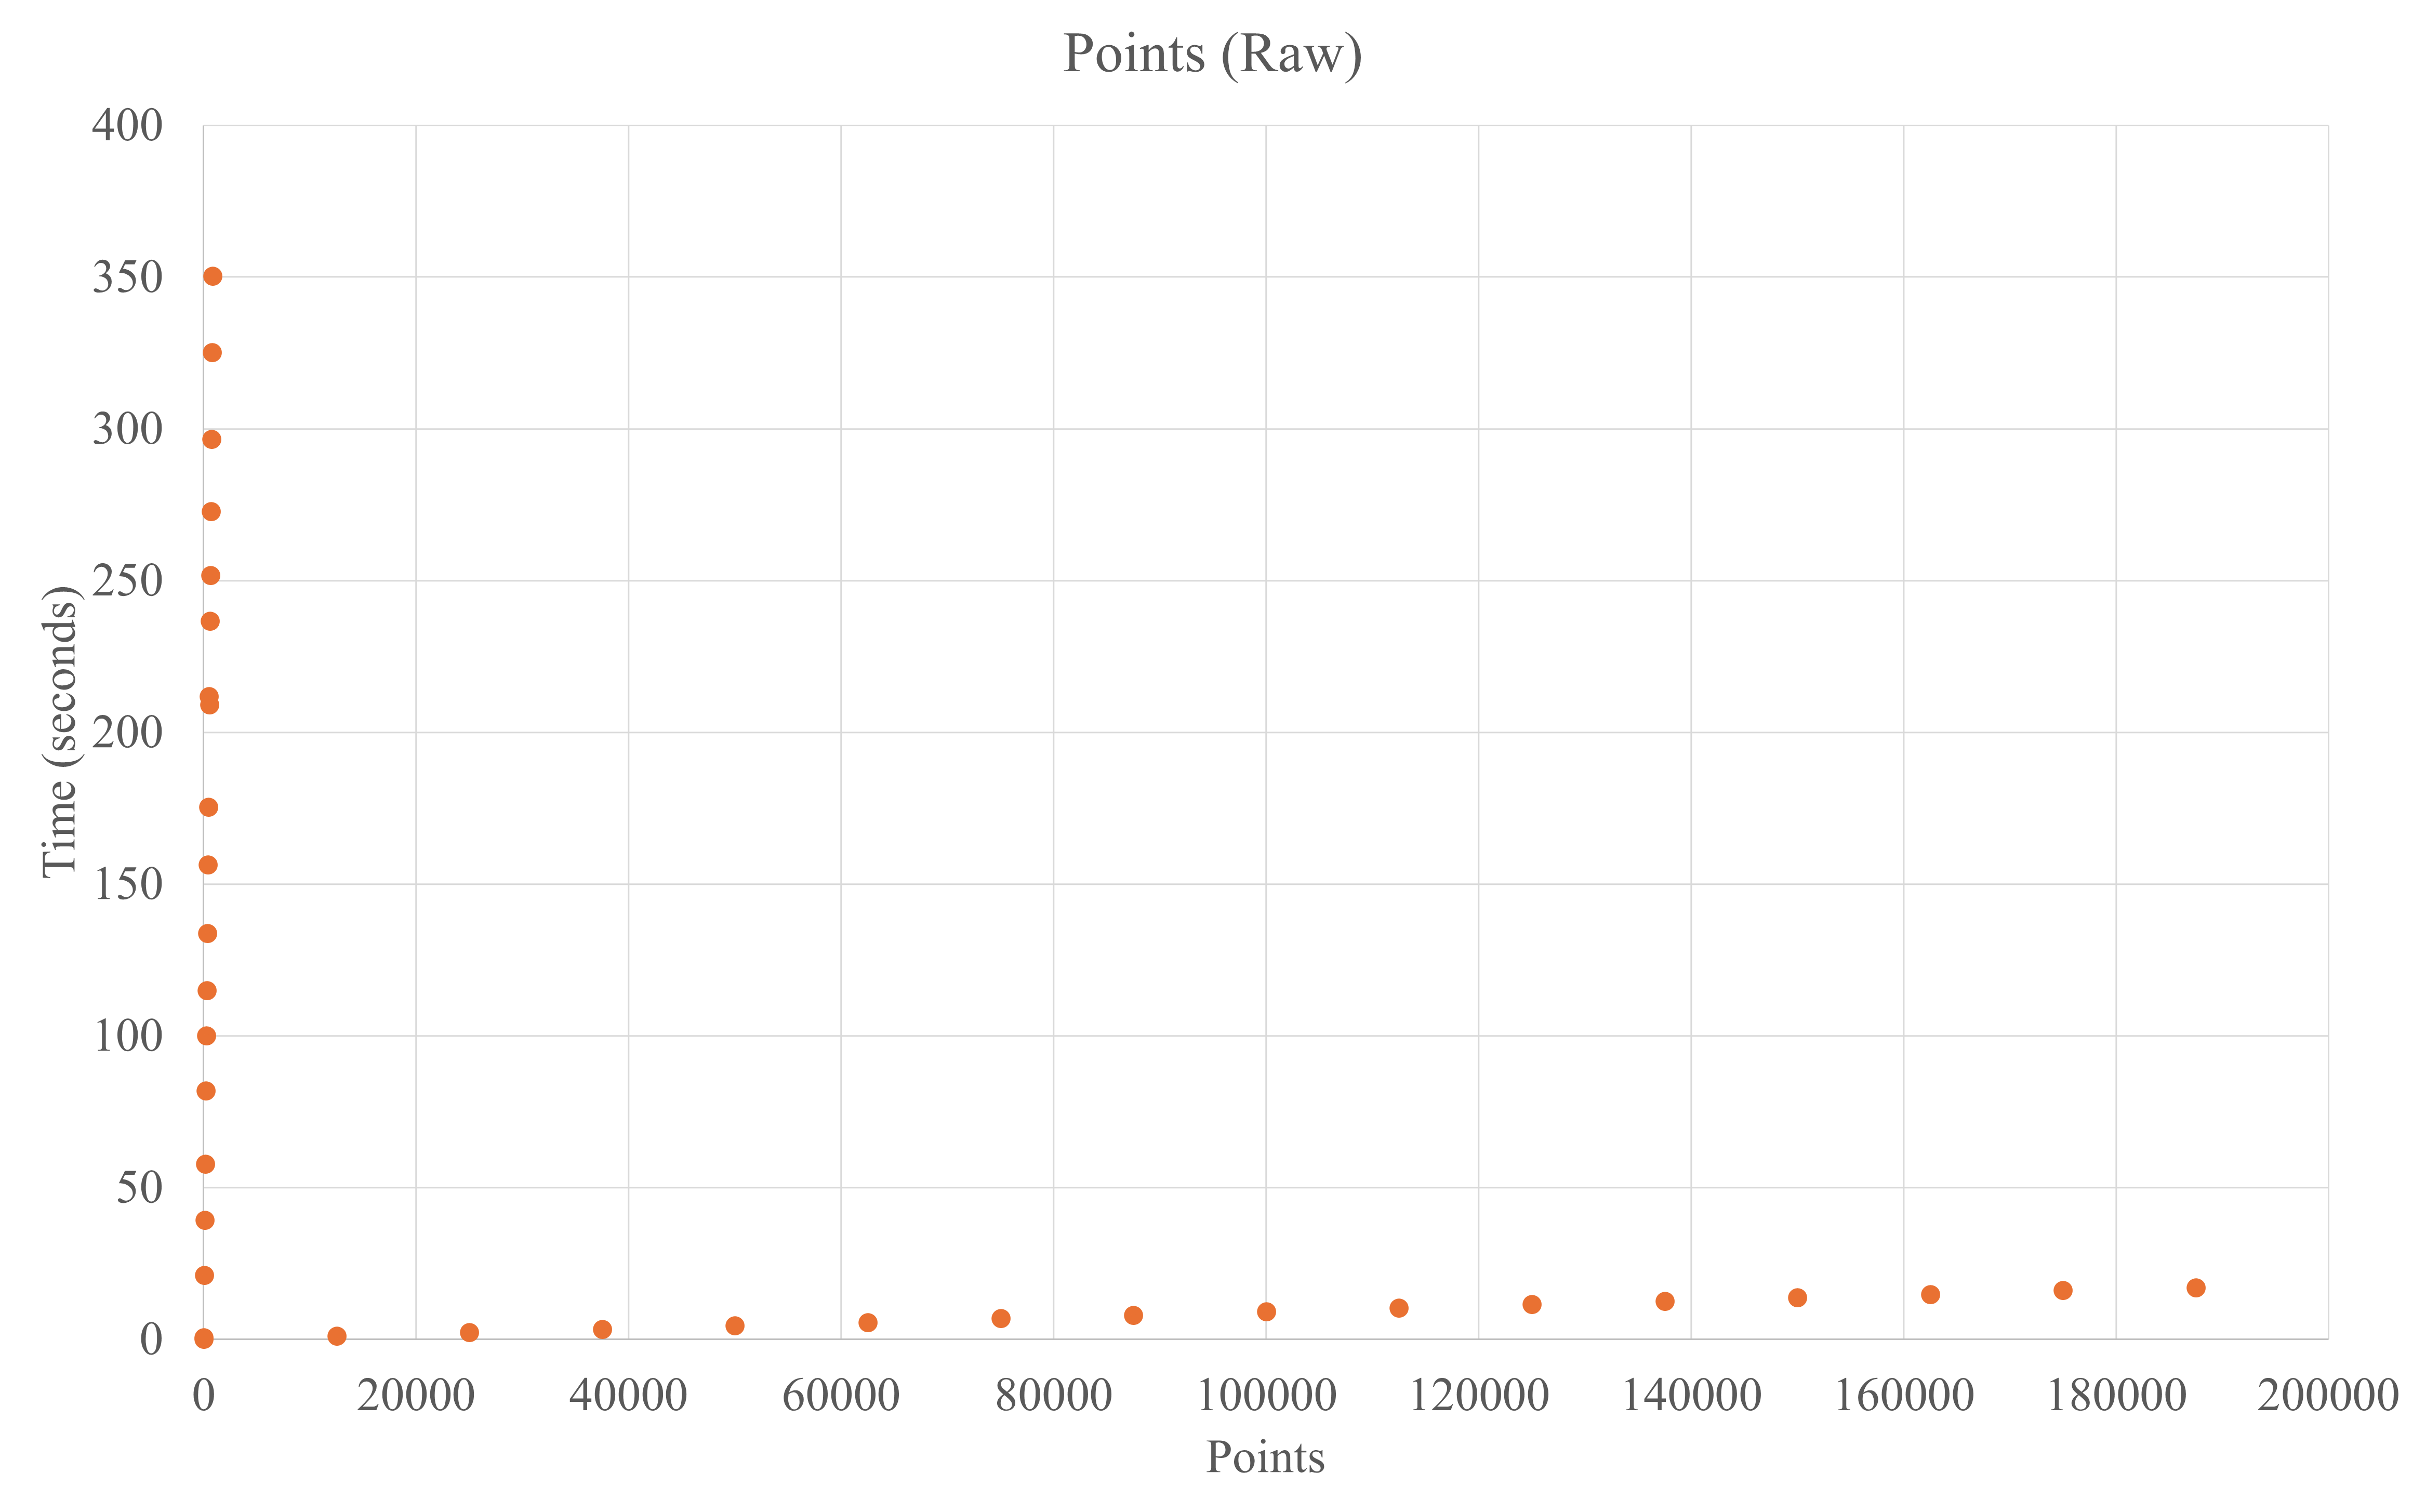
\includegraphics[width=0.45\linewidth]{PointsUnedited.png}}&
        \subfloat[Processed Points]{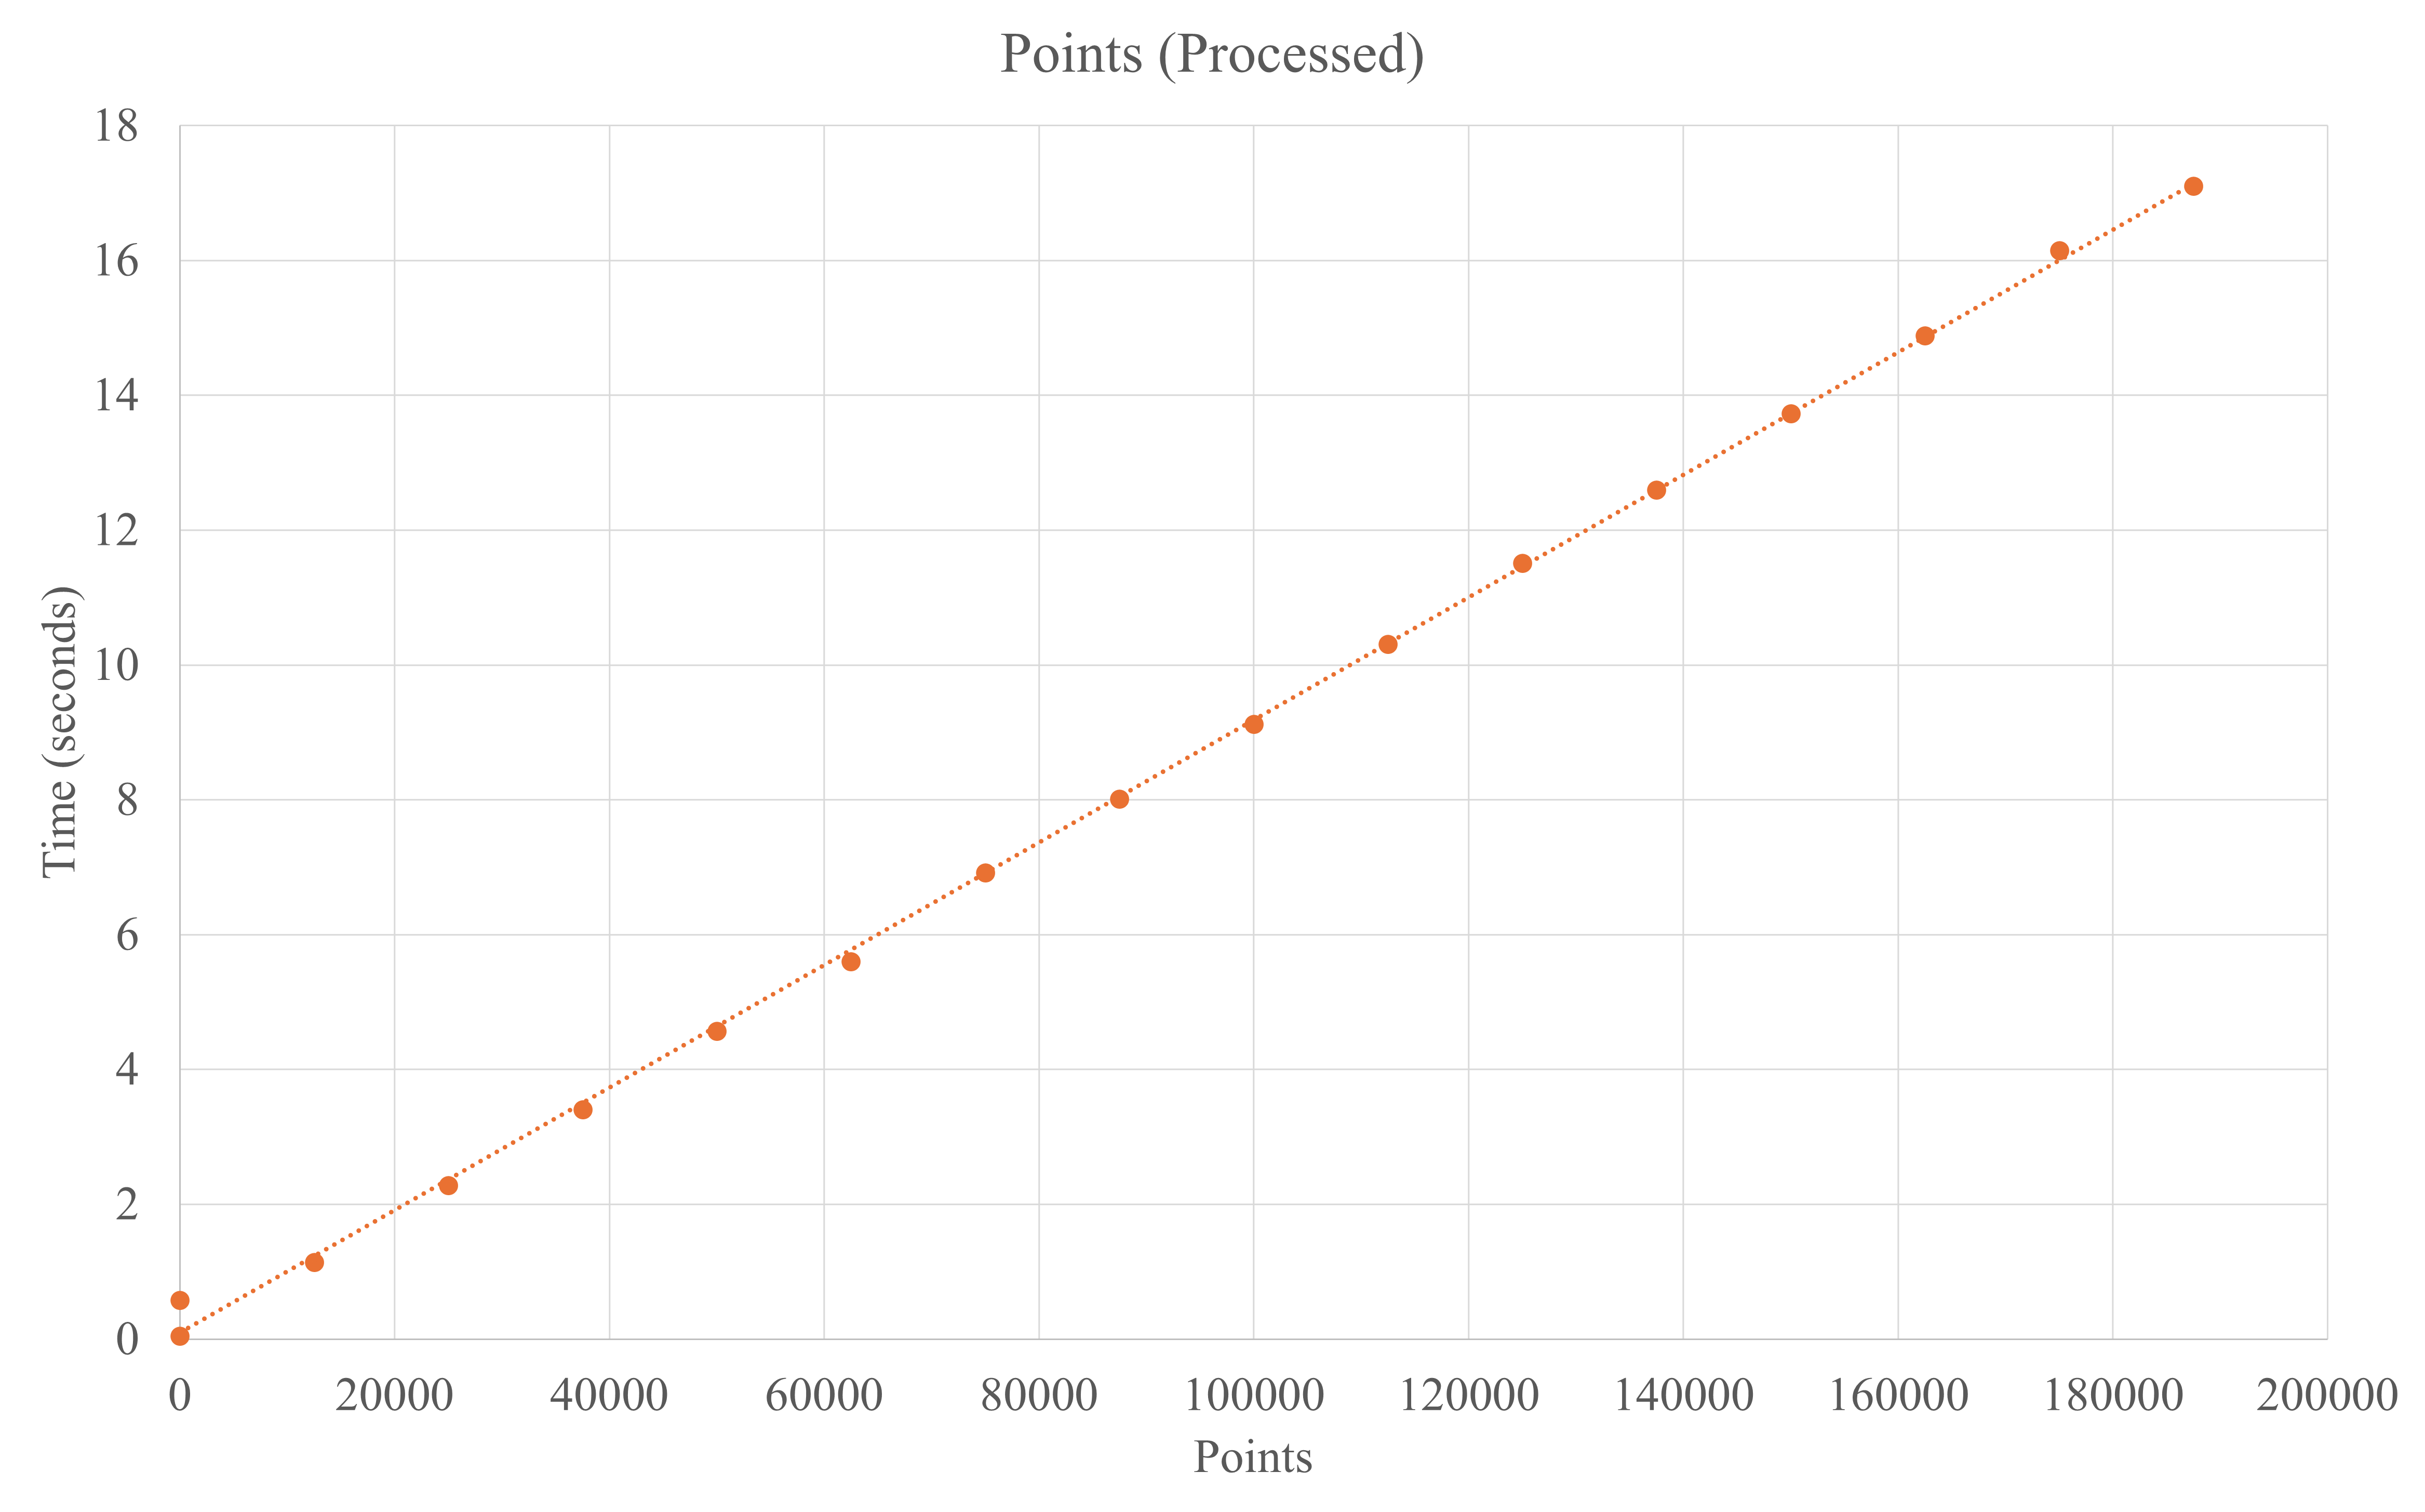
\includegraphics[width=0.45\linewidth]{PointsEdited.png}}
    \end{tabular}
    \caption{Runtime for increasing Points}
    \label{fig:PointsResults}
\end{figure}

\begin{figure}[h!]
    \centering
    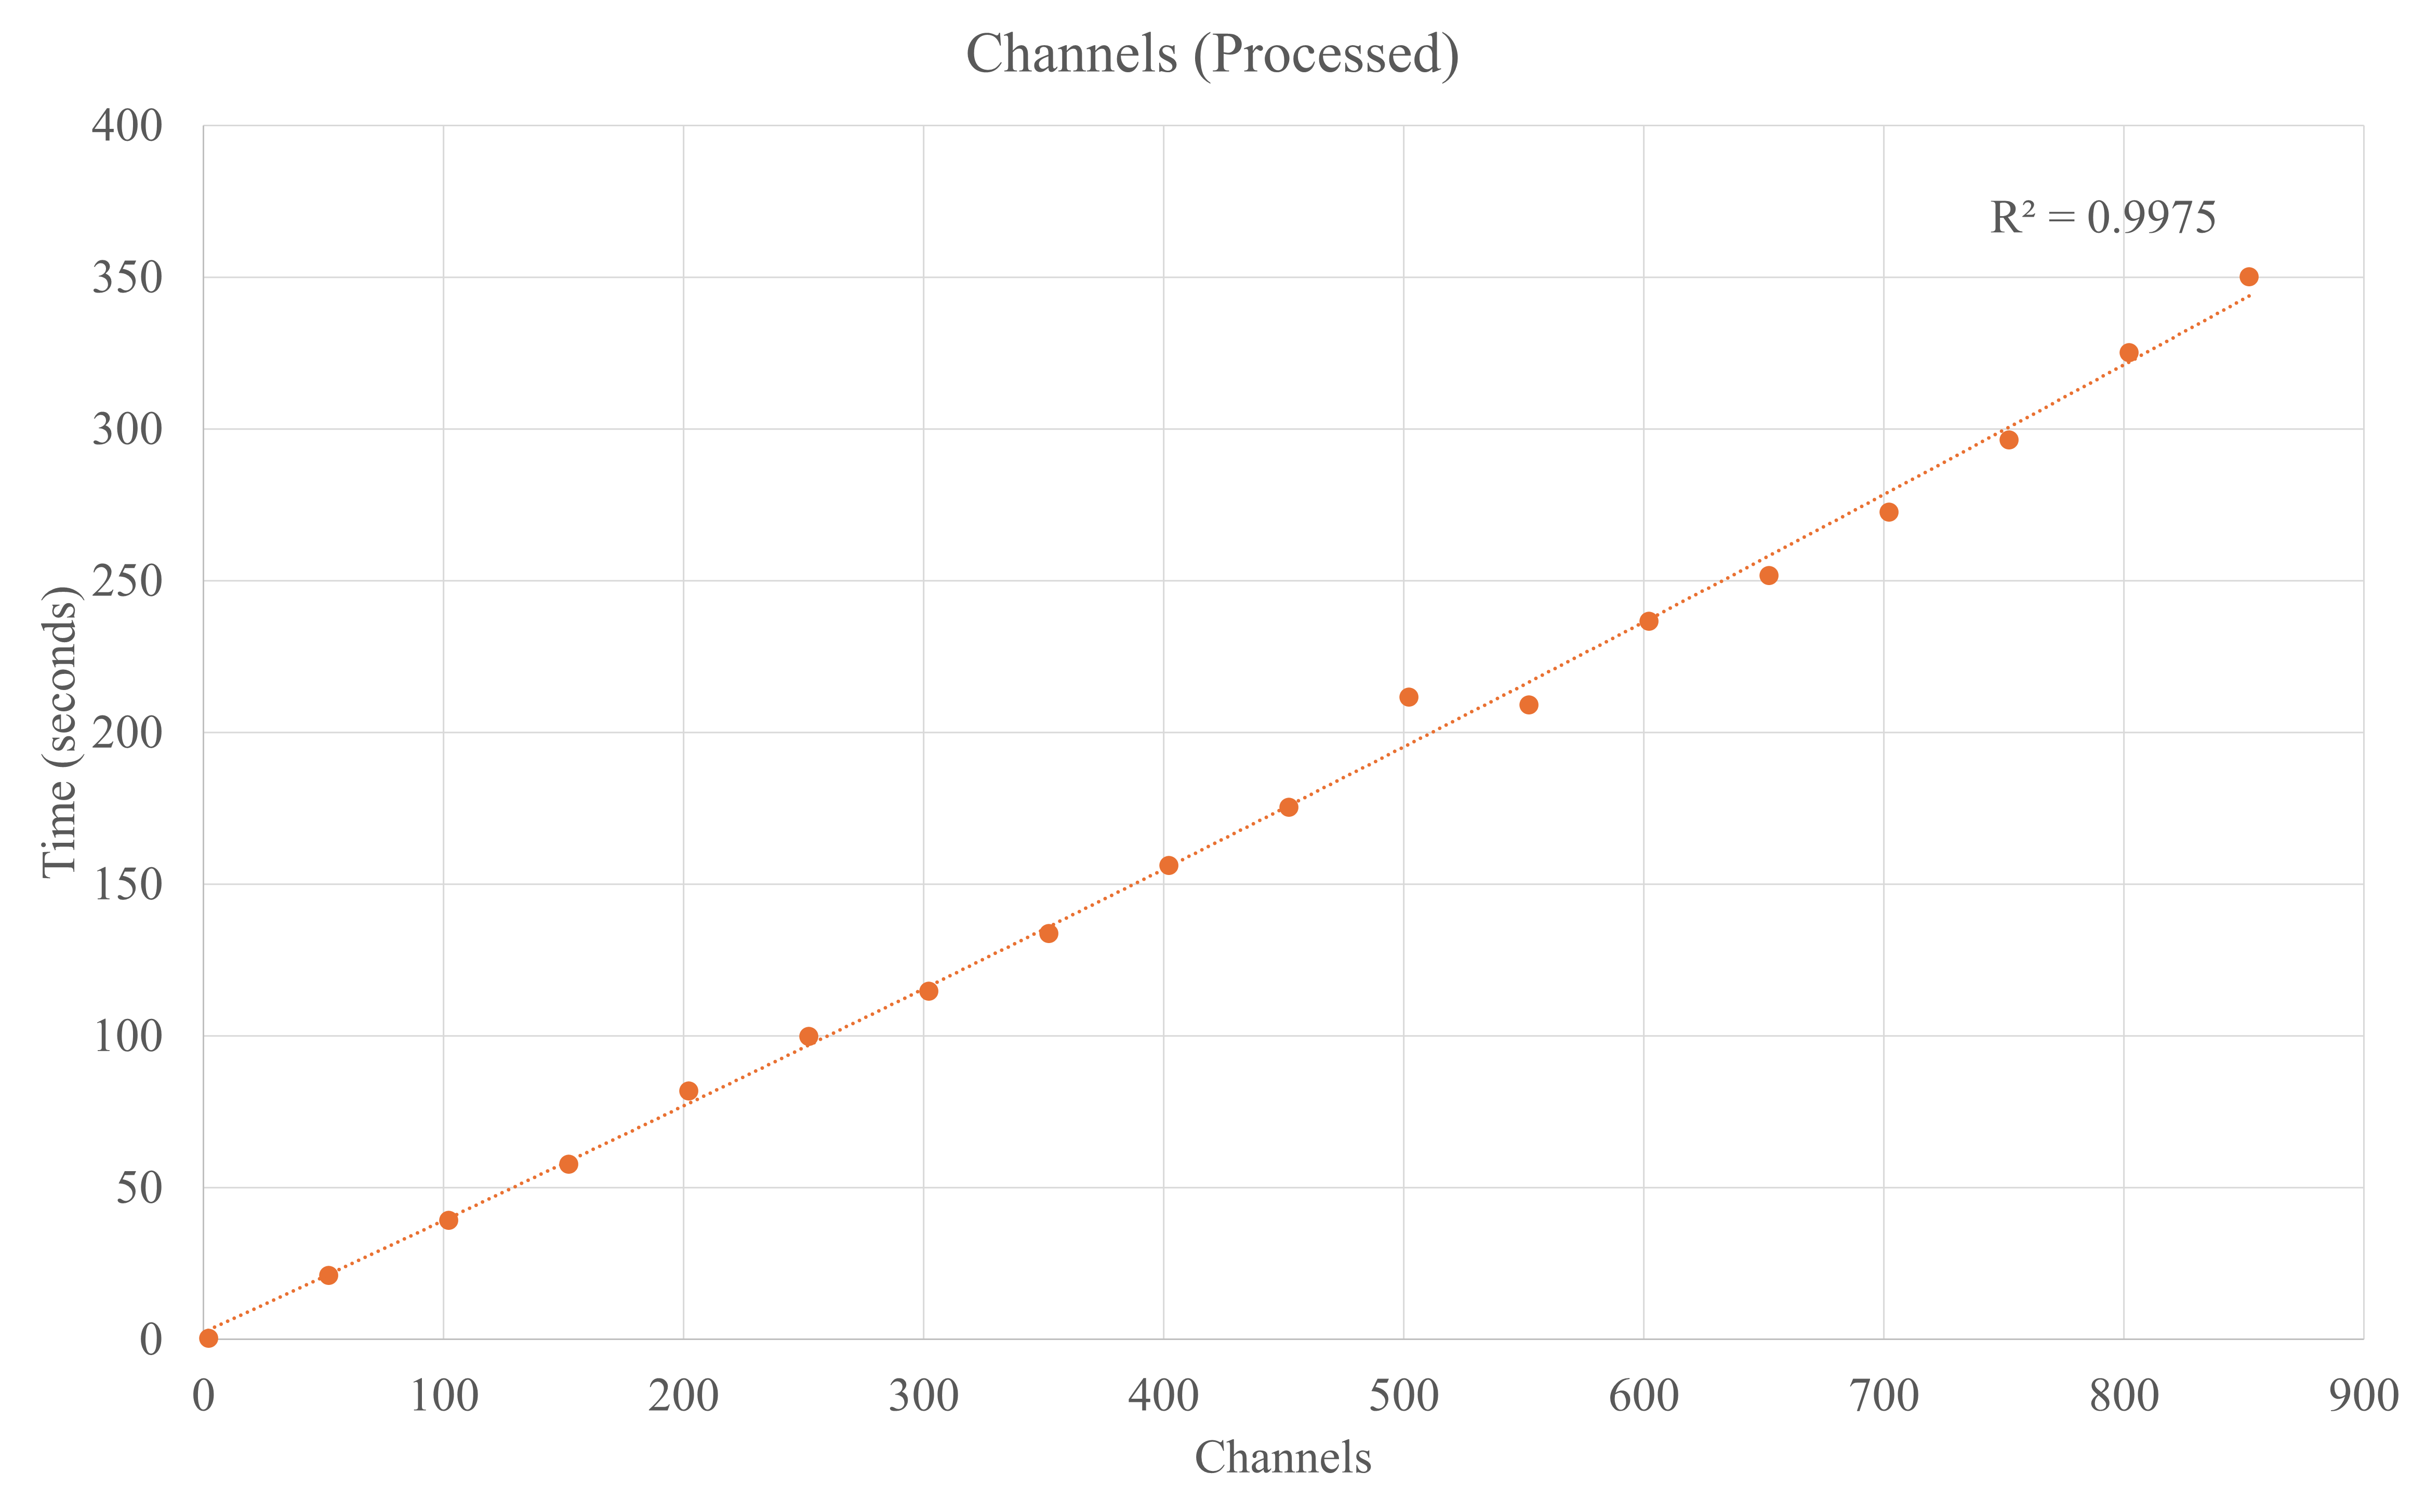
\includegraphics[width=0.75\linewidth]{ChannelsUnedited.png}
    \caption{Runtime for increasing Channels}
    \label{fig:ChannelsResults}
\end{figure}
\vspace{1mm}
\begin{figure}[h!]
    \begin{tabular}{cc}
        \subfloat[Raw Frequencies]{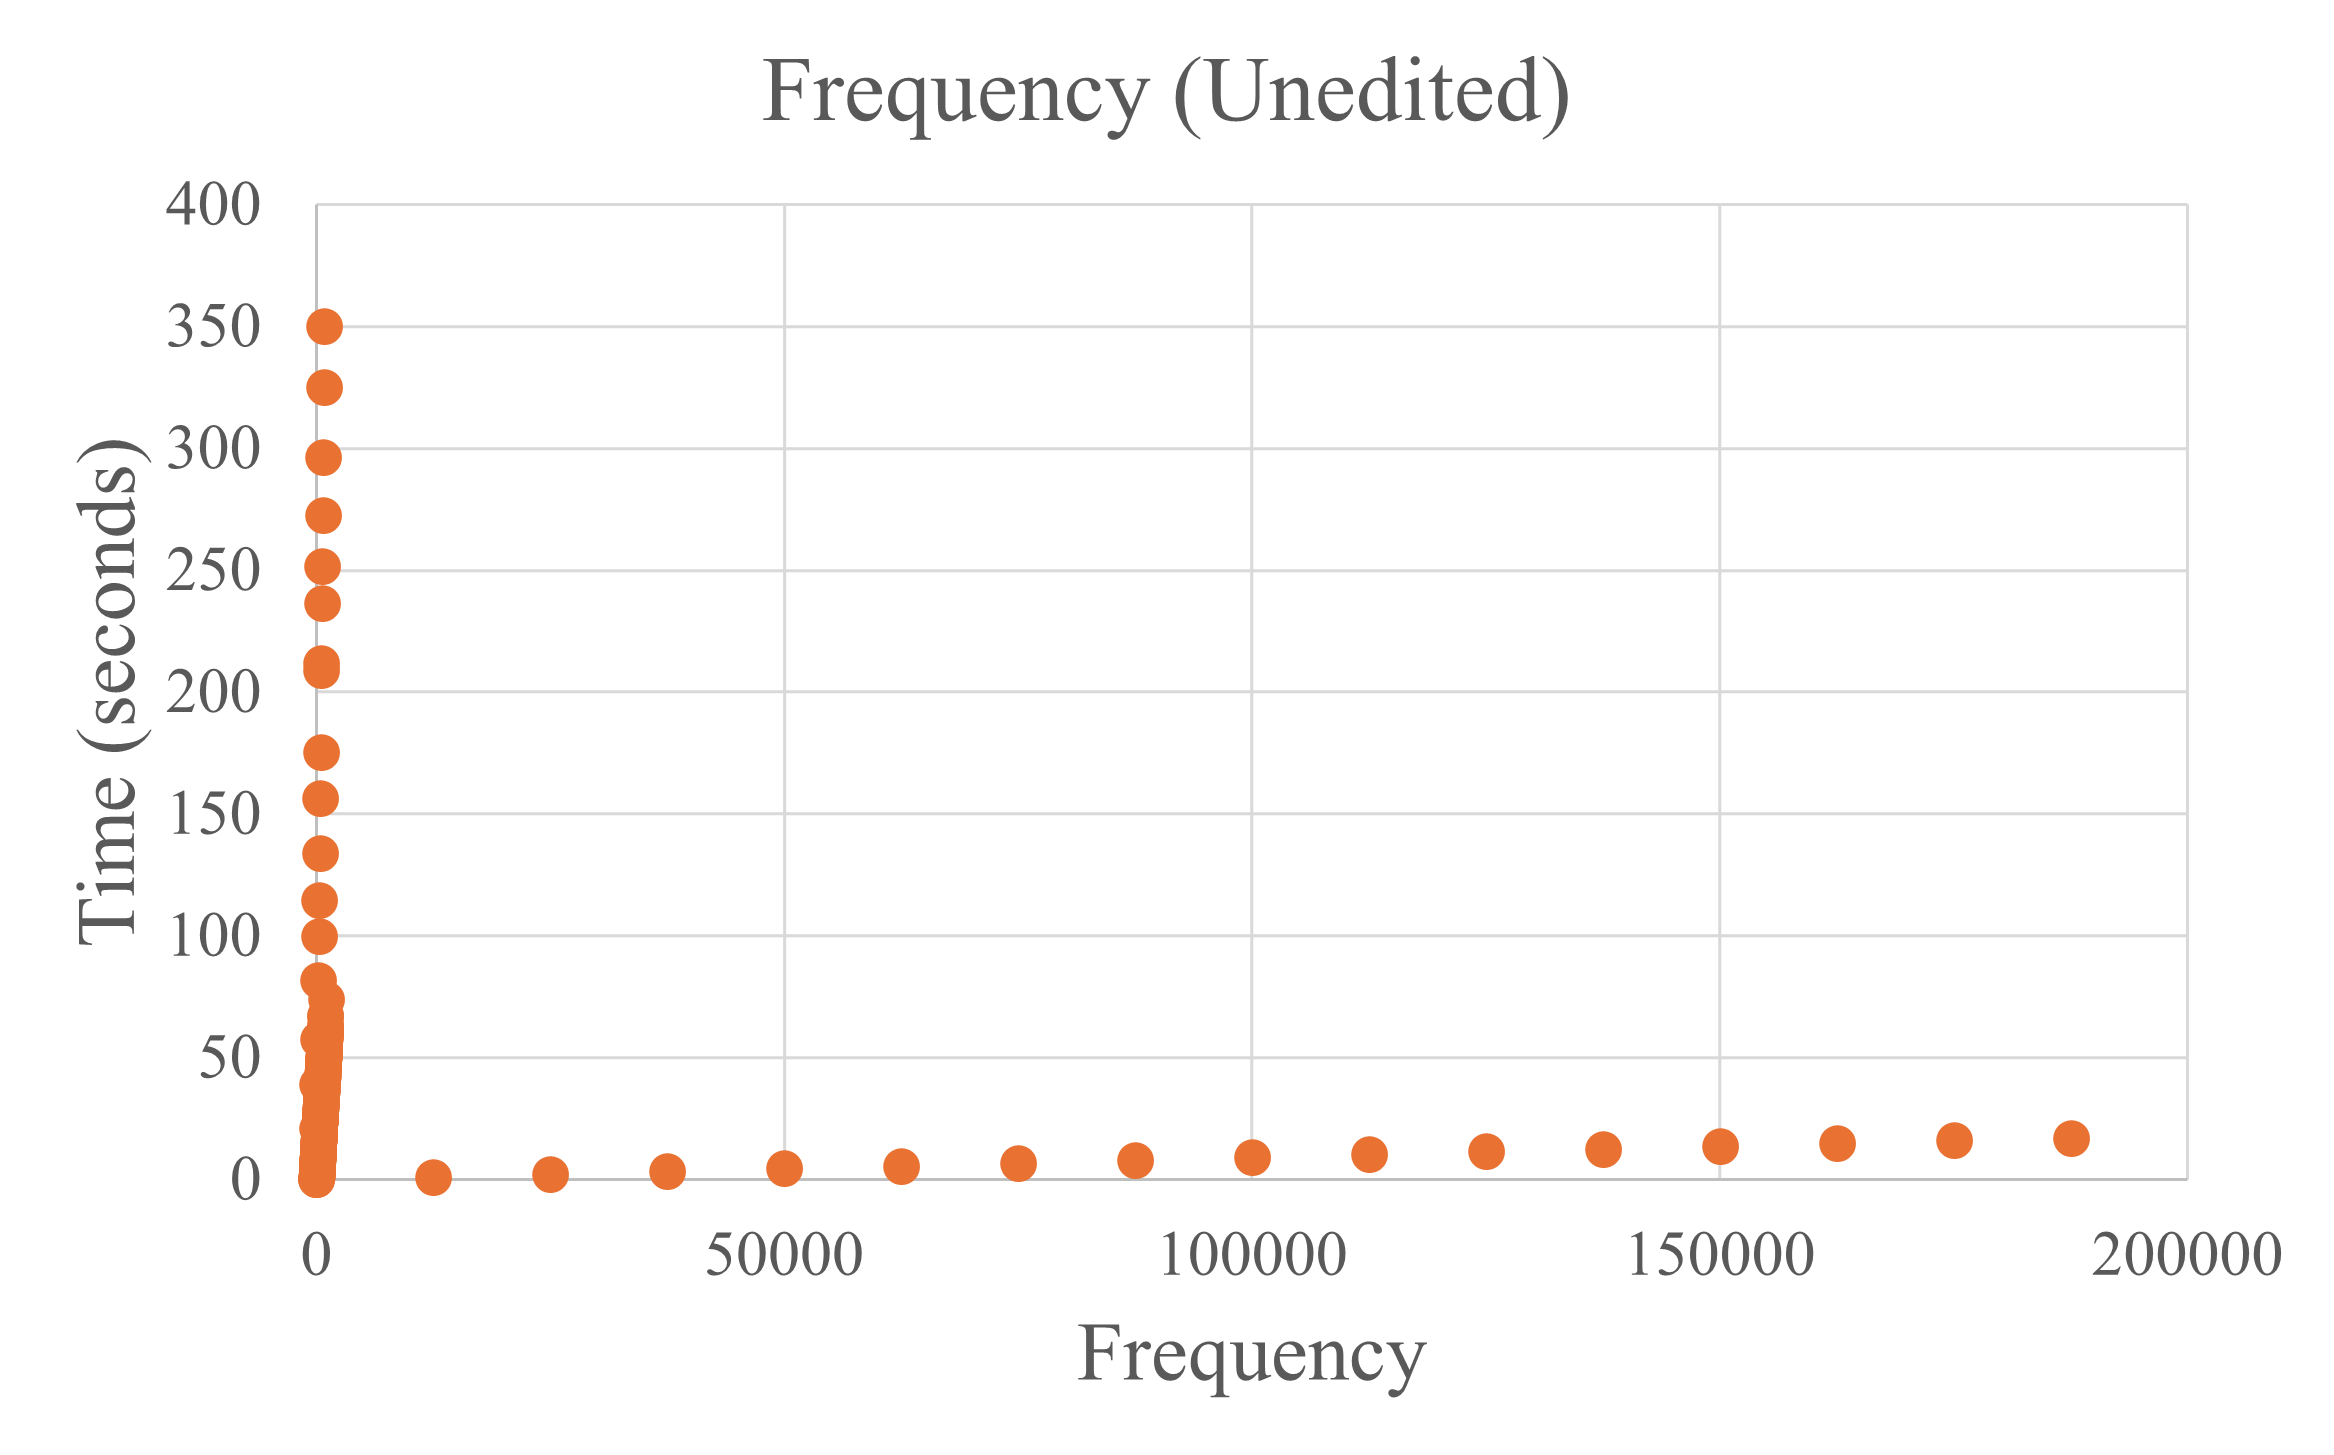
\includegraphics[width=0.45\linewidth]{FrequencyUnedited.png}}&
        \subfloat[Processed Frequencies]{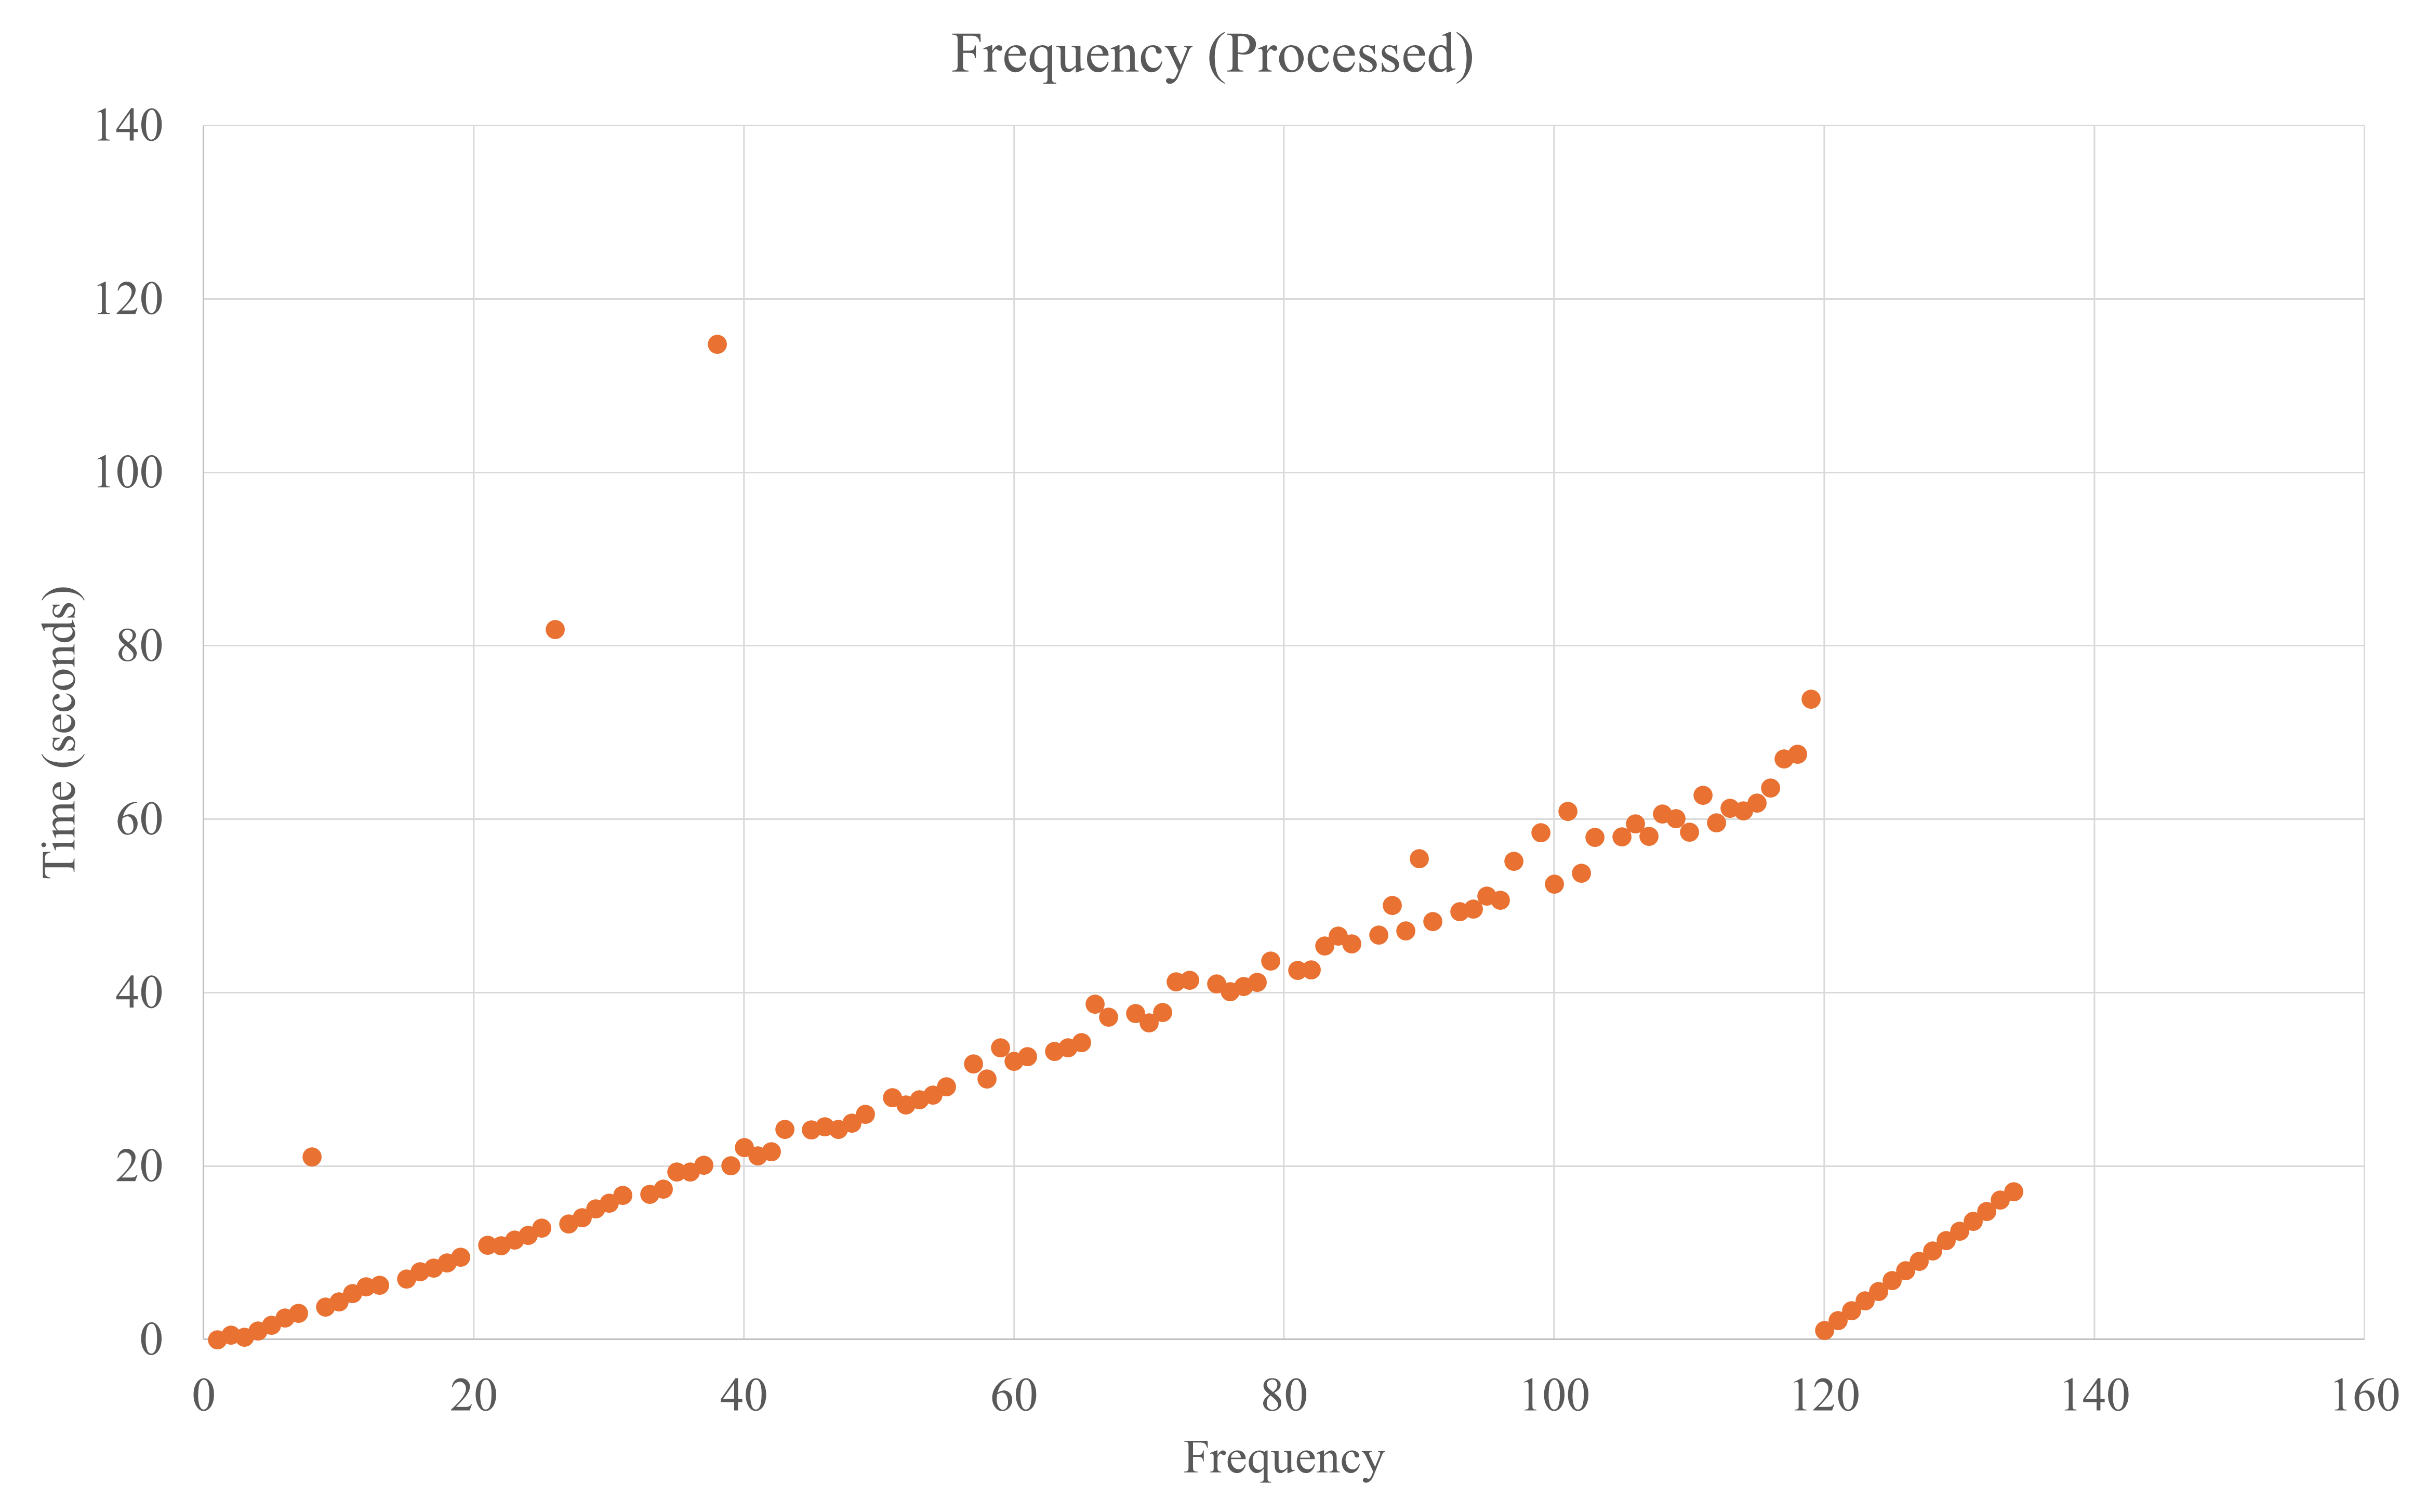
\includegraphics[width=0.45\linewidth]{FrequencyEdited.png}}
    \end{tabular}
    \caption{Runtime for increasing Frequency divisions}
    \label{fig:FrequenciesResults}
\end{figure}

Figures \ref{fig:PointsResults}, \ref{fig:ChannelsResults}, \ref{fig:FrequenciesResults} show the results
from BenchmarkTools. The reason for the two types of graphs was to remove outliers that skewed the data and prohibited
any analysis. Running the benchmark used all the free RAM available on my laptop as well as significant amounts of swap
space on my drive due to large amounts of overhead introduced by the BenchmarkTools benchmark. I believe that the
latency caused by IO to the swap file was the cause for the outliers and so I removed them in the edited graphs since
these points are not indicative of the actual performance of the library. After these points were removed, a curve was
fitted to each graph to provide an indication of the time complexity. From this analysis, I concluded that the runtime
of the library scales linearly ($\mathcal{O}(n)$) with the number of points, and quadratically ($\mathcal{O}(n^2)$) with
the number of channels. This aligns with expectations based on the code analysis of the DAS implementation. The main
beamformer loop consists of a single for loop iterating over the points as such, the algorithm is expected to behave
linearly with an increase in points. With channels, every additional antenna corresponds to a quadratic increase in
channels since every antenna can send to and receive from any other antenna in a fully multistatic system. This is
evidenced by the slight quadratic increase in Figure \ref{fig:ChannelsResults}. The algorithm is expected to have
$\mathcal{O}(n)$ growth since the frequency is only used once in the algorithm process to delay each signal, which is
evidenced by the linear growth in \ref{fig:FrequenciesResults}. Effectively, MERIT works very well with a large number
of points and with relatively few channels. This in turn affected the layout of the matrices in the library. Since data
to do with points would be accessed most frequently, the decision was made to place these along the columns of the
matrices. Since Julia is a column major language, this would provide the quickest access to this data. Data that relate
to the channels were placed along the second dimension since this would be accessed less frequently than data related to
the points. Finally, data relating to the frequency were placed along the third dimension, since this data is accessed
very infrequently, it was decided that the latency required to load this data from memory would be acceptable provided
it allowed us easy access to data relating to points and channels. The above graphs demonstrate the performance of the
MERIT.jl library. From limited testing on my laptop with an Intel i7-1185G7 CPU and 16GB of RAM, the Julia library
executed in the same amount of time as its MATLAB counterpart. However, further testing to accurately quantify the
runtime of both libraries is needed.

\section{MERIT.jl as a Library}
%%Talk about MERIT.jl as a library and talk about how its general. Compare and contrast with Tyson Rheimers python code.
\setcounter{chapter}{5}
\setcounter{section}{0}
\setcounter{subsection}{0}
\chapter*{Future Work}
\addcontentsline{toc}{chapter}{Future Work}
MERIT.jl in its current state already provides researchers with the tools to analyze and visualize scans and through the
integration of the aforementioned programming features, it achieves flexibility and extensibility. This chapter will
consider the scope of future work and how it can be integrated with MERIT.jl

\section{Time Domain Implementation}
\label{TDImplementation}
While this library focused on the frequency domain implementations of the beamformers, equivalent time domain
representations do exist, the main difference being the method in which the signals are delayed. One could extend the \lstinline[language=Julia]{delay_signal!} function in the Process.jl file to
accept signals that are subtyped from the Real abstract type. This way when working with time domain signals, the Julia
compiler, based on the principals of multiple dispatch, will select the correct implementation of the
\lstinline[language=Julia]{delay_signal!} function in a way that is fully transparent to the user. One could also extend
the \lstinline[language=Julia]{get_delay} function in Beamform.jl to accept a sampling rate as well as $\varepsilon$,
using the concept of closure, these variables would be captured and could be used to return the delay in terms of
samples instead of seconds. The functional implementations of the beamformers can stay as they are, as they sum over the
already delayed signals, they are indifferent to the numerical type of the input. 

\section{Implementation of More Beamformers}
The implementation of further beamformers can be an area for future work. Section \ref{JuliaScientificComputing} showed
how the structures and functions from multiple libraries could be combined behind the scenes to provide a more
streamlined experience for the end user. A similar idea could be implemented in MERIT.jl where the beamformers could be
defined in another library that gets used in MERIT.jl. The main benefit of this approach is that users are given the
option to download a ``lightweight'' version of the library with one beamformer if the particular choice of beamformer
does not matter, or they could install the secondary module and have access to a larger suite of beamformers. Another
benefit is that the developers of MERIT.jl need not concern themselves with having to implement all current and future
beamformers. This can be handled by a separate team thereby dividing the workload. Provided this team follows the
template of the DAS beamformer, they can have the guarantee that their function will also work in MERIT.jl.

\section{Parallel Processing}
Parallel processing was not a feature that was explored as it was outside the scope of this thesis. However, there are
areas of the code that have been identified as ``embarrassingly parallel''. These are sections of code that are amenable
to significant acceleration through the use of multithreading and parallel processing. Consider the beamforming equation
in equations \ref{eq:DASBeamformer, eq:DMASBeamformer}. For all of these, the response at each point is calculated
independently of the other points. As such this operation can be easily split across all available threads or even
all available GPU cores, providing exponential increases to the performance of the library overall. The Julia language
provides native support for threaded for-loops through the use of the \lstinline[language=Julia]{Threads.@threads}
macro, which will evenly split the for-loop range across the threads available to the Julia runtime. However, the onus
still lies on the user to ensure that no data race conditions can occur. Julia also supports GPU programming natively
through the use of CUDA.jl for Nvidia GPUs, AMDGPU.jl for AMD GPUs, oneAPI.jl for Intel GPUs as well as Metal.jl for the
current Apple integrated GPUs \cite{JuliaGPU}. However, one drawback to parallel processing is the increased logic
required to collect all the answers at the end. To prevent race conditions when writing to the output array, each
spawned thread would either have to acquire a lock on the final array in order to write to it or pass its calculated
answer to another thread that would sequentially write to the output array. In both cases, the performance provided by
parallelizing the code would be hampered by the overhead introduced by collecting the results. 
\setcounter{chapter}{5}
\setcounter{section}{0}
\setcounter{subsection}{0}
\chapter*{Conclusions}
MERIT.jl was created to answer the question, "
% note that your supervisor may have a strong opinion on the style of referencing you use. Some background is available at https://www.overleaf.com/learn/latex/Bibtex_bibliography_styles
\bibliographystyle{IEEEtran} %Changed to IEEETran by HS
%\bibliographystyle{unsrt}

\bibliography{citations.bib}
\appendix
\renewcommand{\thechapter}{A\arabic{chapter}}


\end{document}